\documentclass[12pt]{report}
\usepackage[utf8]{inputenc}
\usepackage{graphicx}
\usepackage{amsmath}
\usepackage{subcaption}
\usepackage{bbm}


\graphicspath{ {images/} }
\DeclareMathOperator*{\argmax}{\arg\!\max}

\title{
	{A Study of 3D Deformable Parts Models for Detection and Pose-Estimation}\\
	{\large University of Bern}\\
}
\author{Simon Jenni}
\date{March 31, 2015}

\begin{document}

\maketitle

\chapter*{Abstract}
This work covers the implementation of a 3D Deformable Parts Model and provides experimental evaluations of several design choices, model parameters and training-set configurations. A comparison to similar models then shows a performance improvement compared to other 3D DPMs. It also covers the difficulties and methods for incorporating features obtained by Convolutional Neural Networks into a 3D DPM and shows that without fine-tuning of the feature weights, there is no performance gain on cars compared to the standard HOG features.

%\chapter*{Dedication}
%
%\chapter*{Declaration}
%
\chapter*{Acknowledgements}
Foremost I would like to thank my supervisor, Professor Paolo Favaro. His guidance, feedback, constructive criticism, and ideas helped me greatly throughout the work on this project. It was his lecture on Machine Learning that got me interested in this field and I'm very glad for the opportunity he gave me to write my Bachelor's thesis on this exciting topic. I would also like to thank Attila Szab\'{o} who always provided me with great help and advice when I needed it and also taught me many new things. The meetings with Professor Favaro and Attila were always a source of inspiration and motivation and offered me many new insights into the field.

I would also like to thank my family and friends who supported me and provided me with  pleasant distractions from the work on this thesis. I'm especially grateful for the moral and financial support of my father without whom I would not have been able to do this.

A special thanks goes to my very understanding and patient girlfriend C\'{e}line who managed to keep up with me during this time and helped me greatly throughout the writing of this thesis. 


\tableofcontents
\listoffigures
\listoftables

\chapter{Introduction}
\section{Motivation}

One of the main objectives in computer vision is that of recognising instances of an object category (e.g. cars, pedestrians, faces,...) in images or videos. This has many useful applications like cameras that automatically bring faces into focus, video surveillance systems that track certain objects, traffic monitoring, and roboter vision to name just a few. When given an image the goal of a typical object detection system is to list whether one or several instances of a pre-trained object class are present, and to indicate its position in the image via a rectangular bounding box, tightly covering the object instance (see figure \ref{fig:vocEx}).
\begin{figure}
\begin{center}
        \begin{subfigure}[b]{0.49\textwidth}
                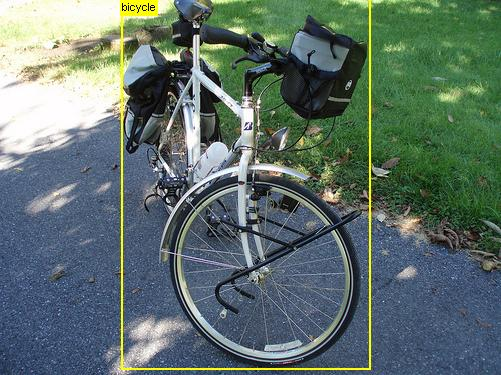
\includegraphics[width=\textwidth]{vocEx1}
        \end{subfigure}
        \begin{subfigure}[b]{0.49\textwidth}
               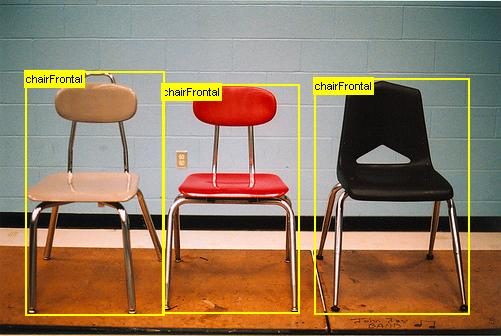
\includegraphics[width=\textwidth]{vocEx2}
        \end{subfigure}
\caption{Examples from the Pascal Visual Object Classes (VOC) challenge 2012. \cite{pascal-voc-2012}}
\label{fig:vocEx}
\end{center}
\end{figure}

Object category recognition remains one of the most challenging goals of computer vision. While for us humans it is mostly a trivial and effortless task, teaching a computer to recognise objects is very challenging. Given an image, all the computer initially "sees" are numbers referring to the RGB values of each image pixel. Today, the arguably most important step towards teaching machines how to see is to translate these pixel values into more meaningful and task-suited representations (features) of  an image. 

An object recognition system has to deal with a lot of variation between object classes (inter-class variability) as well as inside of object classes (intra-class variability). Cats for example are very different from cars in that they are non-rigid, have a furry texture, etc. and the system should be able to identify and discriminate between both. A recognition system for cars has to be able to detect cars of all sorts of different sizes and types and should also be able to recognise them from any viewpoint. 

One of the most widely used and successful approaches to object recognition in the last decade was the Deformable Parts Model (DPM) \cite{5255236}. It combines effective scale-invariant Histograms of Oriented Gradients (HOG) features \cite{1467360} with a deformable geometric model and mixture models that allow it to model intra-class variation effectively for many object classes. Current state of the art results in object detection are achieved by systems based on Convolutional Neural Networks (CNN) \cite{girshick2013rich}, a technique that made an impressive comeback thanks to the possibilities of GPU-programming (which made efficient training possible) and the existence of large datasets \cite{krizhevsky2012imagenet}.

\begin{figure}
\begin{center}
        \begin{subfigure}[b]{0.43\textwidth}
                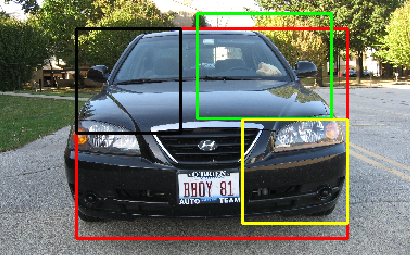
\includegraphics[width=\textwidth]{view1}
        \end{subfigure}
        \begin{subfigure}[b]{0.43\textwidth}
               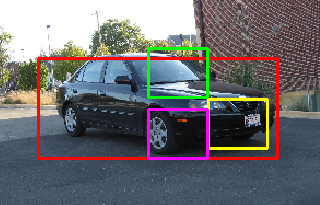
\includegraphics[width=\textwidth]{view2}
        \end{subfigure}
        \begin{subfigure}[b]{0.43\textwidth}
                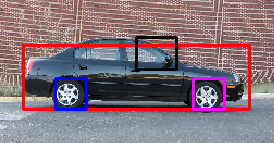
\includegraphics[width=\textwidth]{view3}
        \end{subfigure}
        \begin{subfigure}[b]{0.43\textwidth}
               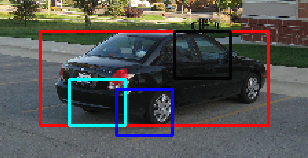
\includegraphics[width=\textwidth]{view4}
        \end{subfigure}
        \begin{subfigure}[b]{0.43\textwidth}
                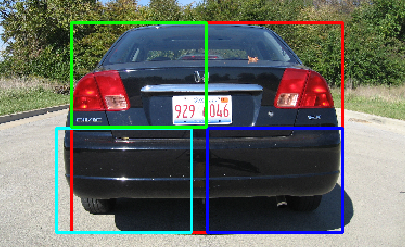
\includegraphics[width=\textwidth]{view5}
        \end{subfigure}
        \begin{subfigure}[b]{0.43\textwidth}
               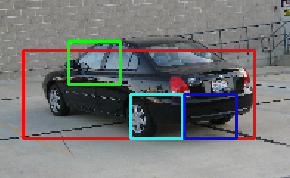
\includegraphics[width=\textwidth]{view6}
        \end{subfigure}
        \begin{subfigure}[b]{0.43\textwidth}
                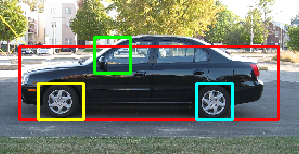
\includegraphics[width=\textwidth]{view7}
        \end{subfigure}
        \begin{subfigure}[b]{0.43\textwidth}
               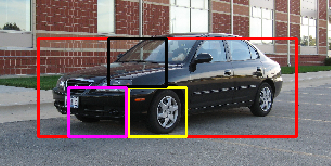
\includegraphics[width=\textwidth]{view8}
        \end{subfigure}                
\caption{This figure shows detections of an eight-viewpoint-3D-DPM with six 3D-parts and three parts per viewpoint. The red boxes indicate the root filter placement and the other boxes indicate part placements. Each 3D part is assigned a separate  colour to help illustrate their consistent 3D placement. Note that this model was trained with a small number of parts for illustration purposes. The images are taken from the 3D Objects Dataset of \cite{4408987}.}
\label{fig:carviews}
\end{center}
\end{figure}

Very often, more information than just the presence and location of an object would be useful. To arrive at a better scene understanding, we might, for example, like to know the viewpoint that an image of an object was taken under. For this reason, there was a recent growth of interest for 3D object representations. The arguably most successful 3D models today are based on the DPM and have delivered impressive results in viewpoint recognition while upholding and in some cases even increasing 2D bounding box localisation \cite{6248075,Pepik:2012aa}. The extension of a DPM to 3D is usually done by anchoring object parts in three-dimensional space and modelling a discrete number of viewpoints. Modelling objects under a set of discrete viewpoints requires to have viewpoint information provided in the training data and introduces additional supervision to the training procedure. It is interesting to note however that a normal 2D DPM very often learns objects under specific viewpoints, therefore justifying the approach of the 3D model. The mapping of the 3D part position to the 2D image plane during test-time is done via a viewpoint dependant projective mapping. Part appearances are learned for each model viewpoint separately, with the constraint that they have to be consistent across views. This is important as otherwise the 3D information of the model reduces to basically just a number of different object views. Figure \ref{fig:carviews} illustrates the consistent 3D learning of part appearances on detections of the 3D-DPM implemented in this project. Detections for the same car are shown for eight viewpoints that the model was trained on. In contrast to detections of a usual 2D-DPM (see figure \ref{fig:dpmcar}), which models parts independently for different views, we observe that the parts detected with the 3D-DPM have a 3D geometric relationship. To enforce the 3D constraints on the model, exact viewpoint information for several views of the same object instance are needed. This information is usually provided by  renderings of Computer Aided Design (CAD) models. 


\begin{figure}
\begin{center}
        \begin{subfigure}[b]{0.49\textwidth}
                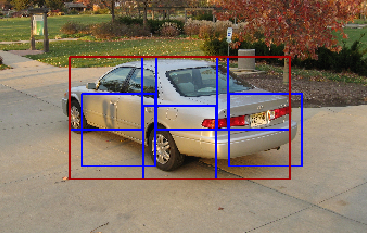
\includegraphics[width=\textwidth]{dpmcar1}
        \end{subfigure}
        \begin{subfigure}[b]{0.49\textwidth}
               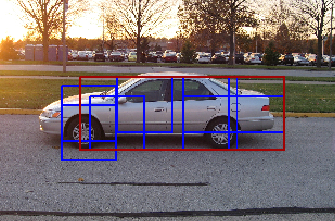
\includegraphics[width=\textwidth]{dpmcar2}
        \end{subfigure}              
\caption{This figure shows detections of a normal 2D-DPM. The red boxes indicate the root filter placement and the blue boxes indicate part placements. Note that there is no apparent connection between parts of the two different views.}
\label{fig:dpmcar}
\end{center}
\end{figure}

The aim of this project is to implement and study a 3D deformable parts model for the detection and pose-estimation of cars. The implementation will be based on the successful and openly available implementation of the original DPM \cite{5255236}. The study will cover the use of new annotated training data, implementation details, an evaluation of model and training parameter choices, experiments on well known and challenging datasets and a comparison to other models. Furthermore, it will also cover the incorporation of features obtained from Convolutional Neural Networks into the model and how these affect the training procedure and the performance of a 3D-DPM. 


\section{Outline}

This thesis is structured into  three main chapters. Chapter \ref{chap:back} provides an overview of the research field at hand and gives a review of related work. Also, a brief introduction to the two image-descriptors (features) used in the project will be given. This chapter sets the context for the research in this thesis.

In chapter \ref{chap:model}, the model implemented in this project will be introduced. In section \ref{sec:dpmreview} a review of the original DPM (on which it is based on) will be  provided and a formal framework for the model will be set up. Section \ref{sec:ext3D} will then explain the modifications made to the DPM to arrive at a 3D object model. Finally, section \ref{sec:cnnFeat} explains the steps taken to replace the HOG features of the original DPM with features obtained from Convolutional Neural Networks.

Chapter \ref{chap:exp} shows and discusses experimental results obtained on several datasets and puts them into context with other work. It also discusses the influence of several model parameters on the model's performance on bounding box localisation and viewpoint estimation.

Finally, chapter \ref{chap:conclusion} will conclude the thesis by providing a review of the results and insights gained throughout the project. It will also discuss ideas for future research work building on this thesis.


\chapter{Background}\label{chap:back}
In recent years, the task of multiple-view object recognition has gained increasing interest in the computer vision community. The combination of object detection and pose-estimation helps to develop a deeper 3D scene understanding which is crucial to several vision goals. 

\section{A Bit of History}
Already in the early days of computer vision, techniques to solve the detection problem were based on 3D modelling. Some of the earliest works in this field were restricted to polyhedral blocks on uniform backgrounds, and approaches relied on edge detectors, line fitting algorithms, and projective projections of feature groupings \cite{books/garland/Roberts63}. The apparent short comings of modelling the world as a "world of blocks" for real world scene reasoning (curves, illumination, complex backgrounds,...) drove forth attempts to model non-polyhedral objects as assemblies of generalised cylinders \cite{agin1972representation}. 

The trend in the 1970s was to model objects as collections of 3D volumetric part primitives. These approaches would often be combined with an elastic arrangement model called "pictorial structures" \cite{fischler1973representation} which served as inspiration to the DPM. 

The 1980s were dominated by exact 3D shape models inspired by CAD models \cite{lowe1987three}. A view-based scheme to represent 3D objects gained momentum during this time: aspect graphs \cite{underwood1975visual}, a network of distinct 2D views of an object. 

In the 1990s a paradigm shift from 3D shape models to image based appearance models happened \cite{murase1995visual}. These view-based models made recognition of arbitrary complex objects possible for the first time (only specific objects that the system was trained on of course). The models were still not scale nor viewpoint invariant though.

To overcome these limitations there was a shift from global view appearance representations to localised representations (parts) that are invariant to scale, translation, rotation, illumination, etc. in the 2000s. These methods were made possible by the development of local scale-invariant features like SIFT \cite{lowe1999object} and HOG \cite{1467360}.

\section{3D Approaches}
Attempts to solve multi-view object class detection can roughly be broken down into three groups. 
The first group builds upon existing 3D object models (CAD for example \cite{flynn1989cad}). In \cite{yan20073d} a 3D feature model is constructed by holographically mapping 2D features from training views to a 3D CAD shape model. \cite{4270070} follows a similar approach using a rough 3D model which gets assigned parts that are consistently localised across views and then learning appearance over these parts. 
Another approach based on 3D CAD models comes from \cite{liebelt2008viewpoint}. Here, CAD models are used to extract features via a filtering procedure which are then used to construct 3D-filter maps to represent the objects appearance and 3D structure. 

The second group consists of 2D object detectors that are combined into a multiview detection system. A first step in this direction was taken by \cite{thomas2006towards}. Those 2D object detectors became increasingly powerful through the introduction of new learning procedures and  the use of object part relations and multi scale pyramids \cite{felzenszwalb2008discriminatively}. The DPM \cite{5255236} can be seen as a member of this group, although the connection from mixture component to viewpoint is not explicit. A well performing example of this group is given by \cite{6248075} (DPM-VOC+VP) where the mixture components of the DPM are connected to discrete viewpoints by training the model on renderings of viewpoint annotated CAD models. In \cite{5206633}, viewpoints are estimated after fine-tuning an initial bounding box assumption and eventually, a classifier is evaluated on both, the estimated bounding box and viewpoint. 

The third group consists of methods to build 3D representations dynamically based on initial viewpoint annotated training data. In the work of  \cite{4408987} and \cite{savarese2008view} object categories are modelled by viewpoint invariant parts that are connected through homographic constraints. 

\subsection{Related work}

The 3D Deformable Parts Models (3D-DPM) studied in this thesis can be seen as a mix between group 1 and 2. They build upon one of the most successful 2D object detector to date, the DPM \cite{5255236}. This way, they are already predestined to perform well in 2D bounding box localisation. Different viewpoints are modelled by a discrete number of different mixture-components. Where they differ from examples of group 2 is in that  they model the parts in 3D and place 3D constraints on them. 

The first 3D-DPM was introduced in \cite{6248075} (DPM-3D-Constraint). They place parts in 3D and map them to 2D via an orthographic projection. By relying on CAD data during training, they learn part-appearances consistently across views. The part-deformations are modelled independently for each viewpoint but are of course also consistently learned thanks to the 3D constraints. The learning problem is rephrased as a structured output prediction problem and the Latent-SVM (L-SVM) formulation of \cite{5255236} replaced by a Structured-SVM (SSVM) objective aimed at optimising for both bounding box overlap and correct viewpoint estimation.

The model of \cite{Pepik:2012aa} builds upon \cite{6248075}. They introduce a 3D deformation model for the parts, modelling the deformation by a 3D gaussian distribution. While making the model slightly more compact through a reduction of parameters that have to be learned, this showed to slightly decrease performance compared to \cite{6248075}. In order to recognise viewpoints at a finer scale,  \cite{Pepik:2012aa} interpolate between the filters of the model at test time. The interpolation factors are proportional to the angular distance between the viewpoint that is being tested and the viewpoints the model is trained on.

The model implemented during this project is most similar to \cite{6248075}. It also relies on CAD data during training but uses photo-realistic renderings instead of gradient-based, non-photorealistic ones as in \cite{6248075} and \cite{Pepik:2012aa}. During training, it also makes use of viewpoint annotations on Pascal VOC 2012 provided by \cite{xiang_wacv14}. Instead of an SSVM objective, the model uses the L-SVM formulation of \cite{5255236} and introduces a penalty term during latent-positive search. Also, this project experimented with the use of Convolutional Neural Network features as a replacement for the HOG features, usually used in the DPM.

\section{Features}
This section gives a brief introduction to the two image features used in this project.

\begin{figure}
\begin{center}
        \begin{subfigure}[b]{0.49\textwidth}
                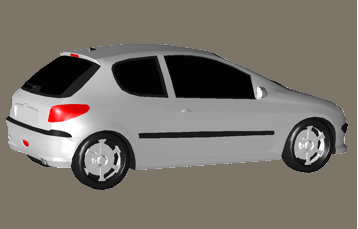
\includegraphics[width=\textwidth]{carnohog}
        \end{subfigure}
        \begin{subfigure}[b]{0.49\textwidth}
               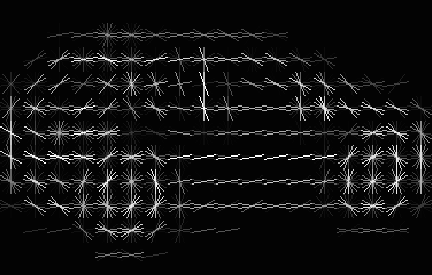
\includegraphics[width=\textwidth]{carhog}
        \end{subfigure}
\caption{Visualisation of a HOG feature map (right) computed from the rendered car image on the left.}
\label{fig:carhog}
\end{center}
\end{figure}

\subsection{HOG}
Histograms of Oriented Gradients (HOG) have been introduced in 2005 by Dalal and Triggs \cite{1467360} and showed remarkable results in pedestrian detection. HOG descriptors divide the image into rectangular cells, compute gradient directions of all the pixels in the cell, and compile a histogram of gradient directions after binning the gradient-votes into typically nine orientation bins. The weight of each gradient vote is given by the gradients magnitude. This accumulation of pixel gradient votes into cells already ensures a small degree of translation-invariance. 

The computed cells are then grouped into overlapping blocks of $3\times3$ cells and local normalisation is performed in each of the blocks. This block normalisation makes the HOG features invariant to changes in contrast and illumination. Each cell leads to a 36-dimensional feature vector. A visualisation of a HOG feature map computed on a rendered CAD car model can be seen in figure \ref{fig:carhog}.

HOG features, with some modifications, are the typical image descriptors used in DPMs. In \cite{5255236} Felzenszwalb et al. proposed a modification of the HOG features which computes both, directed and un-directed gradients and reduces the dimensionality of the features by projecting them on a 31 dimensional subspace.  This variant of the original HOG feature is the standard image-descriptor used in 3D-DPMs.

\begin{figure}
\begin{center}
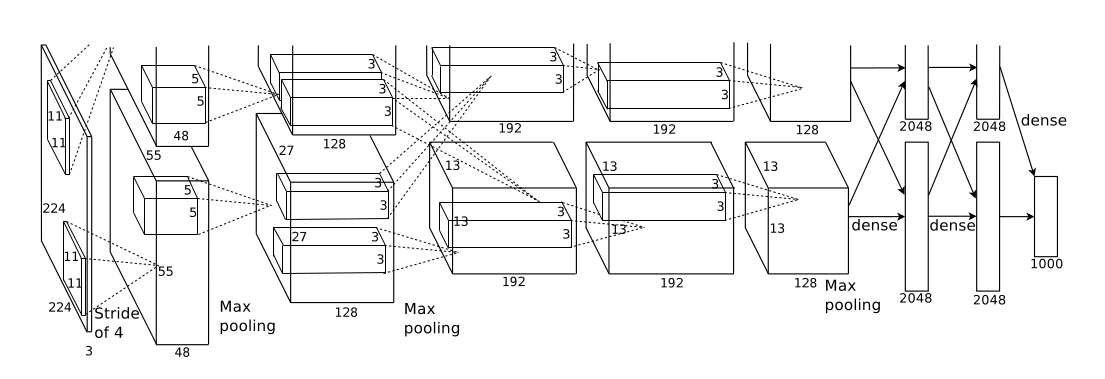
\includegraphics[width=\textwidth]{cnnimagenet}
\caption{Figure showing the architecture of the CNN of Krizhevsky et al. \cite{krizhevsky2012imagenet}}
\label{fig:cnn}
\end{center}
\end{figure}

\subsection{Convolutional Neural Networks}
Recent state of the art performance in image classification and object detection have been reported by methods relying on Convolutional Neural Networks (CNN) \cite{krizhevsky2012imagenet}\cite{girshick2013rich}. CNNs are inspired by biological mechanisms of the visual system and were first introduced in 1980 by \cite{fukushima1980neocognitron}. Their design has since been refined and first promising results on document recognition were reported by LeCun \cite{lecun1998gradient} in 1998 with the introduction of LeNet5. In 2012 Krizhevsky et al. \cite{krizhevsky2012imagenet}  demonstrated the power of CNNs on image classification by showing a substantial improvement in accuracy compared to previous methods.

The architecture of the CNN from \cite{krizhevsky2012imagenet} can be seen in figure \ref{fig:cnn}. CNNs are build out of several types of layers: 
\begin{description}
\item[Convolutional Layers:]  
These consist of several convolution kernels per layer (96 in the first layer of \cite{krizhevsky2012imagenet}). The image is convoluted with each kernel and the result passed on to the next layer. The convolution kernels are not fixed but learnt during training. 
\item[ReLu Layers:]  
The ReLu layer introduces non-linearities into the CNNs and consists of a function that is applied to each of the layer's inputs. The ReLu function is $f(x)=\max(0,x)$, which has shown to considerably reduce training time compared to other functions typically used to model a neuron's output (e.g. $f(x)=tanh(x)$).
\item[Max Pooling Layers:]  These layers partition the input into a set of rectangular subregions and outputs the maximum value of each  subregion, therefore ensuring small translation invariance of the features.
\item[Fully Connected Layers:] These are the last few layers of a CNN. In these layers all the layer's neurons are connected  to all the next layer's neurons. Here is where the high level reasoning of the CNN happens. 
\end{description}

As mentioned before, the filters of a CNN are trained rather than handcrafted. CNNs, as feed-forward networks, are trained  using  backpropagation. Backpropagation works by  back propagating the partial derivatives of the error along the layers. First, the partial derivative of the error with respect to the last layers weights  is computed and the weights updated before the partial derivative for the second-to-last layer is computed and so forth. Once partial derivatives for all the weights have been computed, gradient descent can be used to learn the network. 

There have been very recent reports on the incorporation of  features from Convolutional Neural Networks into DPMs by \cite{girshick2014deformable} and \cite{savalle8deformable}. They both report a substantial improvement in mean average precision on VOC 2007. It is important to note however that cars are an exception to this rule, as CNN feature-based DPMs did not improve on HOG feature-based DPMs on cars. Both \cite{girshick2014deformable} and \cite{savalle8deformable} use the first five layers of the network of Krizhevsky et al.  \cite{krizhevsky2012imagenet} but use fine-tuned weights as provided by \cite{girshick2013rich}. While \cite{girshick2014deformable} do not use the detection fine-tuned weights of \cite{girshick2013rich}, it is unclear which weights were used by  \cite{savalle8deformable}. 

One aim of this project is the incorporation of CNN features into a 3D-DPM, and to study how it affects the performance and training of the model. While the detection performance on cars is likely to decrease compared  to a HOG based 3D-DPM as in \cite{girshick2014deformable}, it is unclear how CNN features affect the model's performance on pose-estimation.

\chapter{The Deformable Parts Model}\label{chap:model}
This chapter will give a review of the Deformable Parts Model as described in \cite{5255236}  and its implementation (VOC-release 3) on which this project builds upon. Section \ref{sec:ext3D} will then introduce the modifications that were made to extend it towards 3D. Wherever possible notation used in \cite{5255236} and \cite{6248075} will be adopted.

\section{DPM Review}\label{sec:dpmreview}
The DPM is a type of sliding window detector, consisting of a set of linear filters which are applied to a feature pyramid computed from an input image. Each DPM has a root filter which models the object appearance as a whole, and several higher resolution part filters which model smaller parts of the object. 

\subsection{Sliding Window Approach}
The idea behind the sliding window approach is that, given an input image and a window (of smaller size than the image), the window is placed on all locations inside the image and  for the region covered by the window to decide whether the object is present or not. 

Rather than working with images directly, feature maps are computed from them. A feature map G is a two-dimensional array of $d$-dimensional feature vectors. One can think of each feature vector as representing a small image patch and the feature map as a grid of feature vectors computed from image patches. The features used in \cite{5255236} are a modified version of the HOG features introduced in \cite{1467360}.
For now let us look at the case of a model consisting of a single root filter (e.g. a DPM without parts).  A root filter F is a two-dimensional array of $d$-dimensional weight vectors. The root filter can be interpreted as the "window" that slides through each position on the feature map to detect objects. 

To detect objects at different scales, a feature pyramid is used (see figure \ref{fig:pyra} and the appendix for a detailed description). The subsampling factor from level to level is constant and determined via a parameter $\lambda$ which fixes the number of levels in an octave. A feature map an octave beneath in the pyramid is computed at twice the resolution.

\begin{figure}[]
\begin{center}
        \begin{subfigure}[b]{0.49\textwidth}
                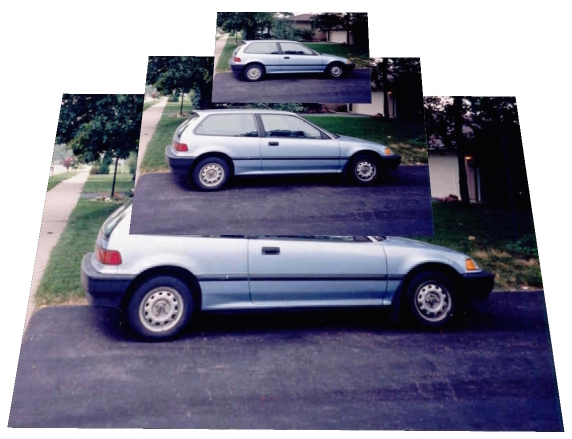
\includegraphics[width=\textwidth]{imagepyra}
                \caption{Image pyramid}\label{fig:impyra}
        \end{subfigure}
        \begin{subfigure}[b]{0.49\textwidth}
               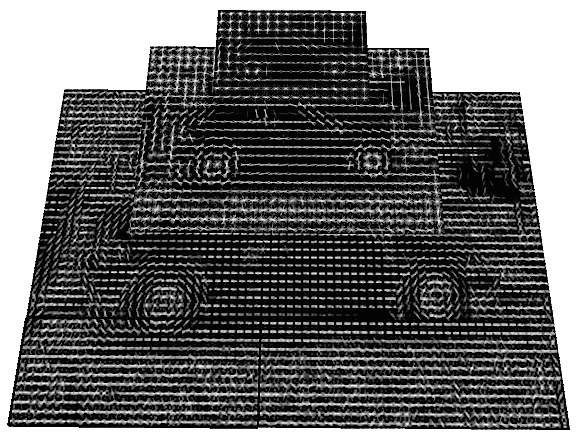
\includegraphics[width=\textwidth]{pyrahog}
               \caption{HOG feature pyramid}\label{fig:featpyra}
        \end{subfigure}
\caption{These figures illustrate image and feature pyramids. The pyramids here span two octaves with one level each. Therefore each pyramid level downwards doubles the image resolution. Note that the cell-size of all the feature maps in the HOG pyramid is constant.}
\label{fig:pyra}
\end{center}
\end{figure}


Each placement of the filter in the feature pyramid is assigned a score via the "dot"-product of the filter and the corresponding sub-array of the feature map at the given level. More formally: given a filter $F$ of size $w\times h$, a filter placement in the feature pyramid is defined by a three-tuple $p=(x,y,l)$ where $(x,y)$ specifies the position of the upper-left corner of the filter in the $l$-th level of a feature pyramid $H$. Further let $\phi (H,p,w,h)$ denote the vector obtained by concatenating the feature vectors in $H$, belonging to a window of size $w\times h$ at position $p$ in $H$.  The score of this placement is then given by:
\begin{equation}
score(p)=F' \cdot \phi (H,p)
\end{equation}
where $F'$ denotes the concatenation of the weight vectors in $F$ and $\phi (H,p)$ is a shorthand for $\phi (H,p,w,h)$, as $w$ and $h$ are implicit from $F$. 

\begin{figure}[]
\begin{center}
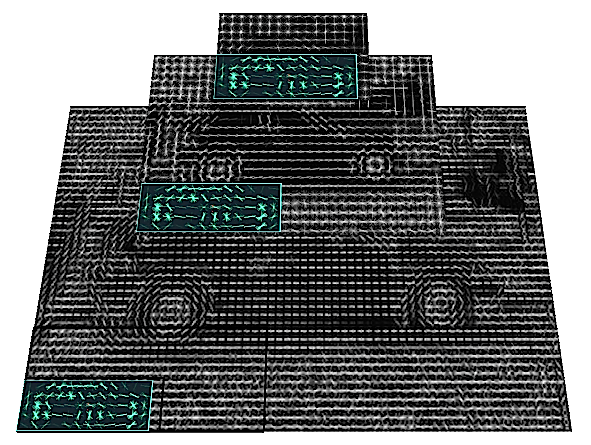
\includegraphics[width=0.6\textwidth]{rootInPyra}           
\caption{This figure illustrates the instantiations of a filter in a feature pyramid. The same filter is placed in the lower left corner of each pyramid level. To better distinct it from the feature maps, the filter is coloured. }
\label{fig:rootInPyra}
\end{center}
\end{figure}
 
\subsection{Deformable Parts and Mixture Models}\label{sec:defParts}
We will now extend the root-only model with parts and a deformation model. Let us consider the case of a DPM model for cars. The root filter approximately covers all of the car and models the object appearance as a whole. It also serves as a detection window. Part filters cover smaller, more detailed parts of the car, e.g. the tires or windows, and model their appearance at a higher resolution. The part filters are always placed $\lambda$ levels (an octave) below the root filter in the feature pyramid and are therefore computed at twice the resolution. Each part is placed at a fixed anchor-position relative to the root filter's position. This leads to a star-shaped model. To model intra-object class variations, parts  are allowed to deviate from their anchor positions by a certain amount restricted by a deformation cost.

Formally, a model with $n$ parts is defined by $(F_0,P_1,...,P_n,b)$ where $F_0$ is the root filter, $P_i$ is a model for part $i$, and $b$ is a bias term. $P_i$ in term consists of $(F_i, v_i, d_i)$ where $F_i$ is the part filter, $v_i$ specifies the anchor position, and $d_i$ is a four-tuple of coefficients for a quadratic  function modelling the deformation cost. A placement $z=(p_0,p_1,...,p_n)$ of all the filters in the feature pyramid is called a hypothesis. The displacement of the parts relative to their anchor position is given by $(dx_i,dy_i)=(x_i,y_i)-(2(x_0,y_0)+v_i)$. Remember that the parts are computed at twice the resolution of the root, hence the factor of two. Figure \ref{fig:anchor} illustrates part anchors and deformations.  Given the displacements, the deformation feature is set to $\phi_d (dx_i,dy_i)=(dx^2,dx,dy^2,dy)$. A hypothesis is assigned a score via
\begin{equation}\label{eq:score}
score(z)=\sum_{i=0}^n F'_i\cdot \phi(H,p_i)-\sum_{i=1}^n d_i\cdot \phi_d (dx_i,dy_i)+b.
\end{equation}
Note that the first term of the sum is concerned with the appearance and the second term with the deformation. 

\begin{figure}[]
\begin{center}
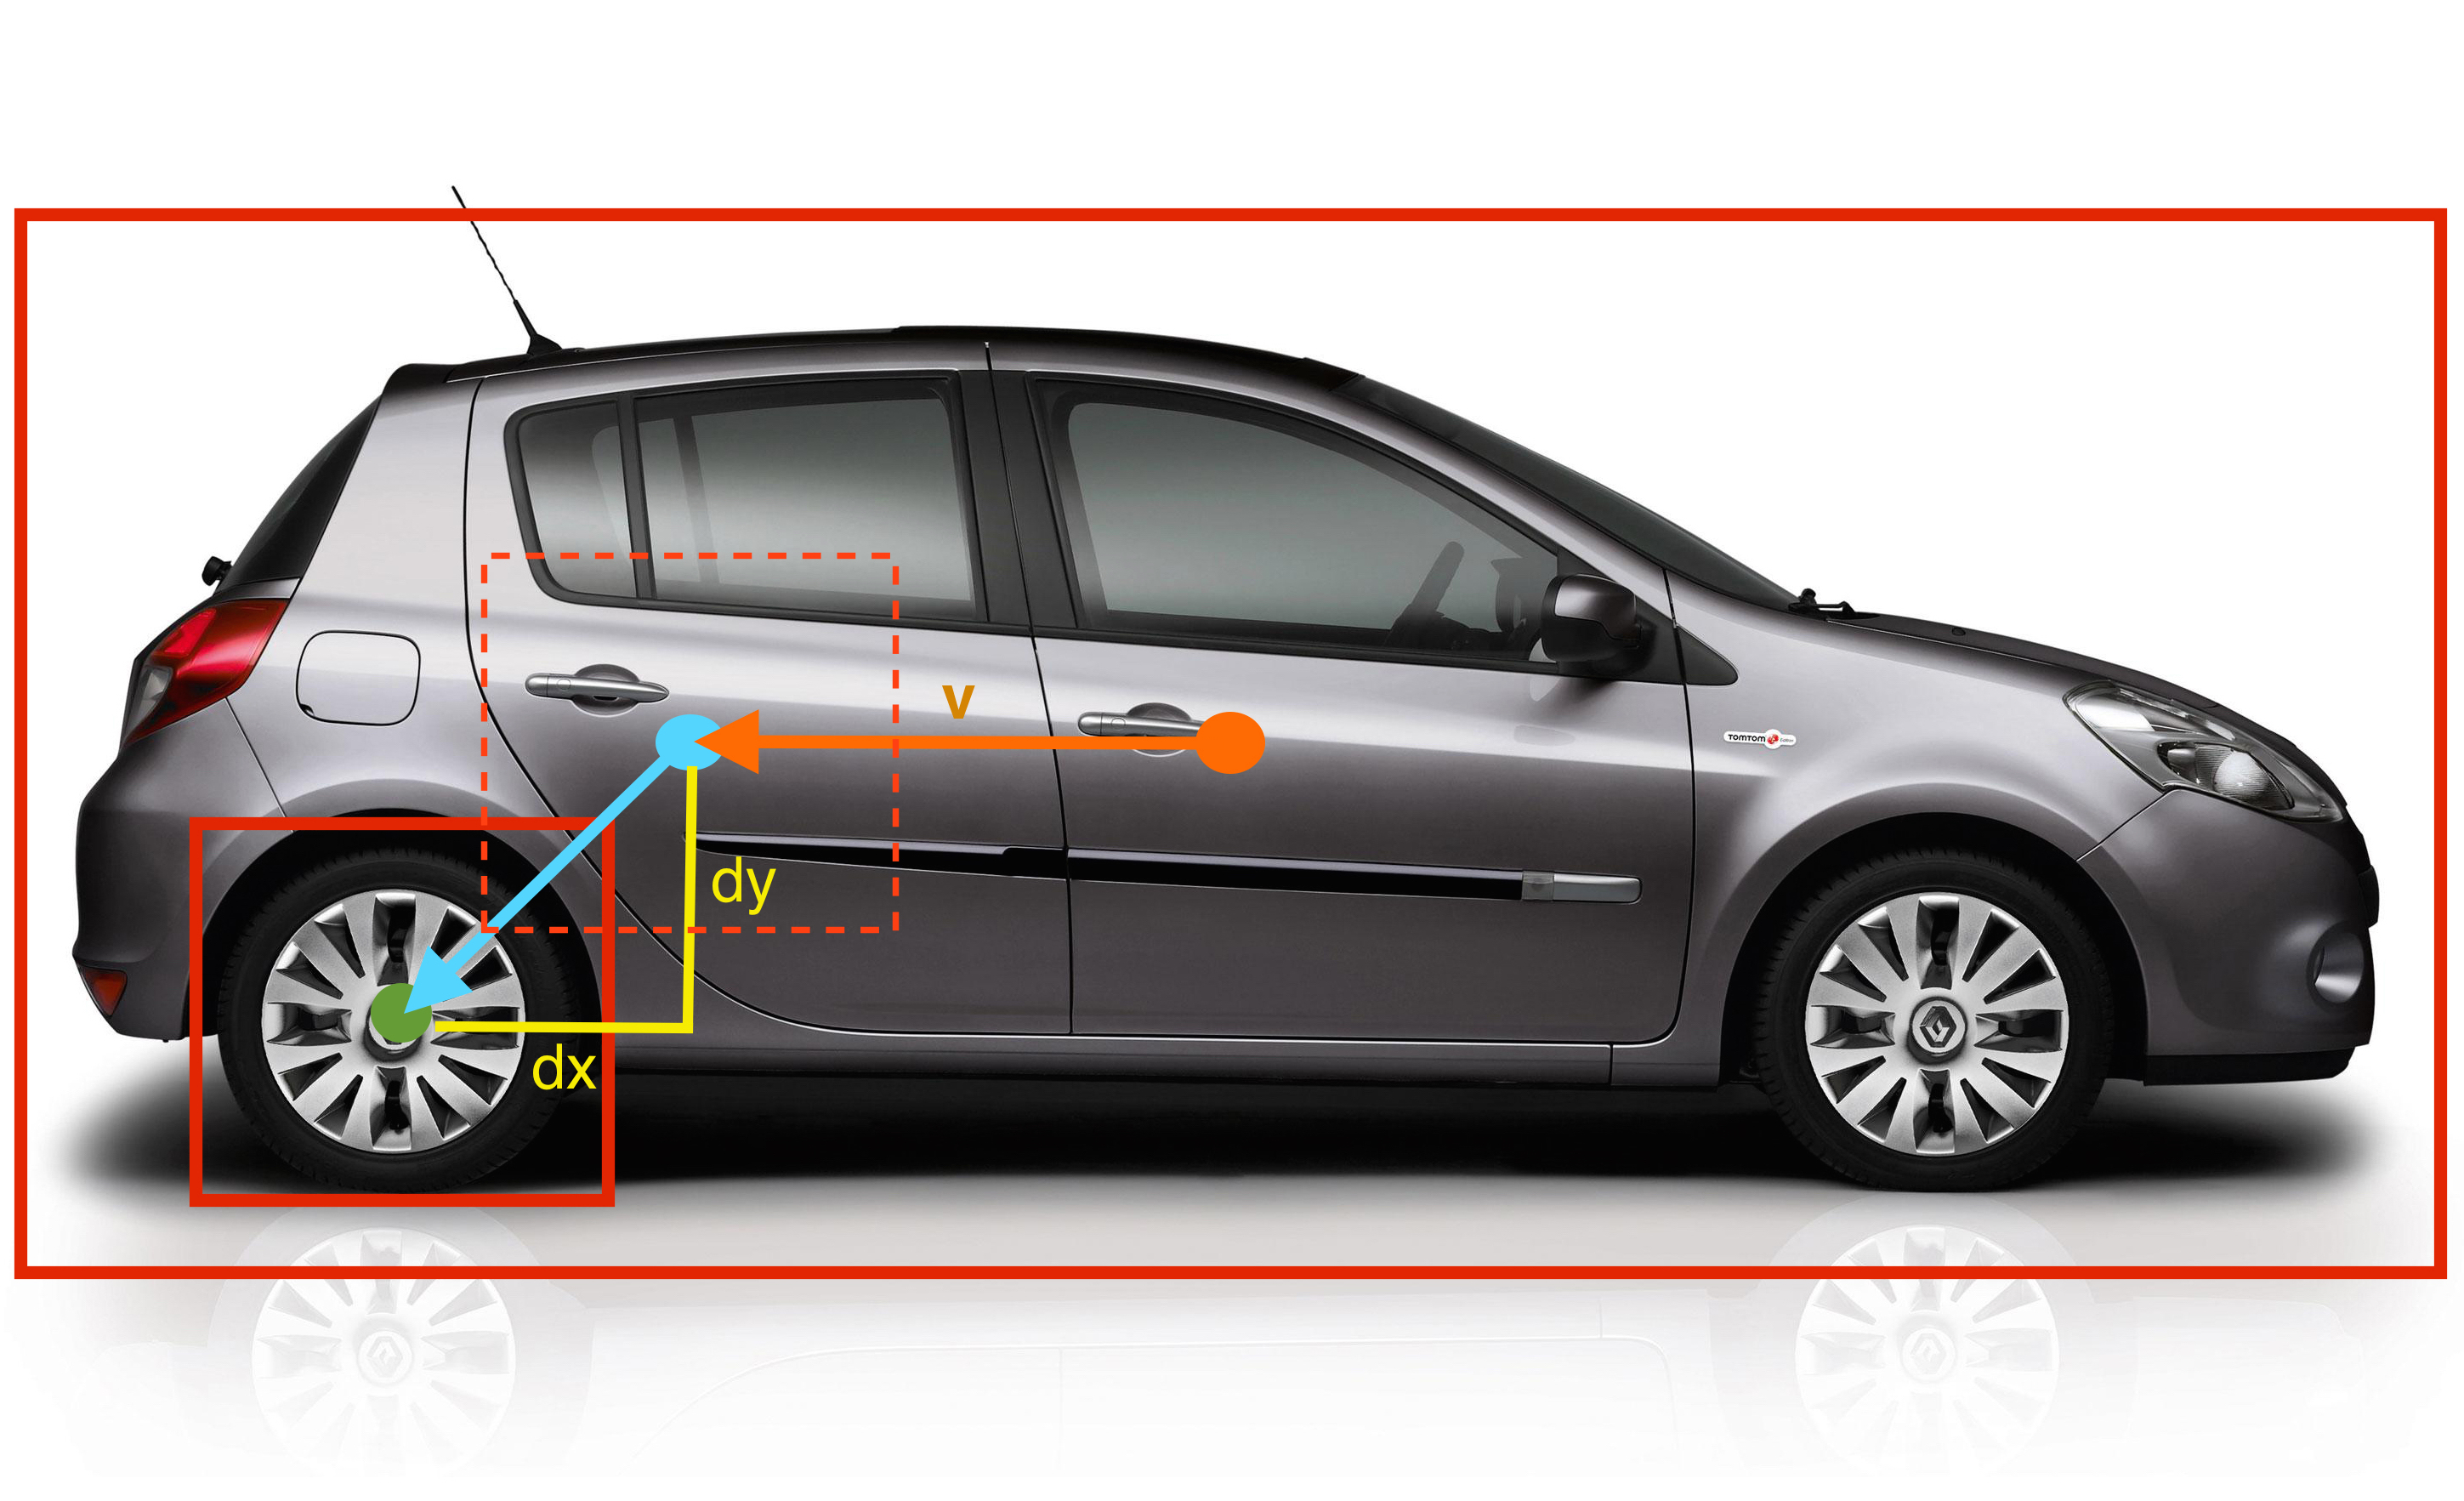
\includegraphics[width=0.8\textwidth]{anchor}           
\caption{This figure illustrates the anchors and displacements of the parts. The anchor position $v$ from the root centre  to the anchor is coloured in orange. The displacement from anchor to the part position is coloured in light blue.  }
\label{fig:anchor}
\end{center}
\end{figure}

To arrive at richer object models, several DPMs, as just described, are combined into one mixture model. A mixture model is an $m$-tupel $M=(M_1,...,M_m)$ where $M_c$ is the model for mixture-component $c$. An object hypothesis for a mixture model is given by $z=(c,p_0,...,p_{n_c})$ where $n_c$ specifies the number of parts in $M_c$ and the score for hypothesis $h$ is simply the score of $z'=(p_0,p_1,...,p_{n_c})$ for $M_c$.

By concatenating all the model-parameters of $M_c$ into a vector 
\begin{equation}
\beta_c=(F_0,F_1,...,Fn,d_1,...d_n,b)
\end{equation}
the whole mixture model can be  expressed through the vector $\beta=(\beta_1,...,\beta_m)$.
By similarly concatenating all the features of hypothesis $z'$ into a vector
\begin{equation}
\Phi(H,z')=(\phi(H,p_0),...,\phi(H,p_n),-\phi_d(x_1,y_1),...,-\phi_d(x_n,y_n),1)
\end{equation}
a sparse feature vector for hypothesis $h$ can be constructed by setting 
\begin{equation}
\Phi(H,z)=(0,...,0,\Phi(H,z'),0,...,0).
\end{equation}
The score of the hypothesis h can then be expressed via the dot product
\begin{equation}\label{eq:vecscore}
score(z)=\beta\cdot \Phi(H,z).
\end{equation}

\subsection{Inference}

As the root filters act as detection windows, the problem of object detection reduces to finding high scoring root placements. The score of a root placement for a mixture component is given by
\begin{equation}\label{eq:rscore}
score(p_0)=\max_{p_1,...p_n}score(p_0,p_1,...p_n).
\end{equation}
That is, for each root placement we want to find the best placements of all the parts. In practice, this is solved by first pre-computing the filter responses and storing them in an array $R_{i,l}(x,y)=F'_i\cdot\phi(H,(x,y,l)$ where $i$ specifies the filter and $l$ the level in the feature pyramid. The filter responses are then transformed via 
\begin{equation}\label{eq:dt}
D_{i,l}(x,y)=\max_{dx,dy}( R_{i,l}(x+dx,y+dy)-d_i\cdot\phi(dx,dy)).
\end{equation}
$D_{i,l}(x,y)$ gives the maximum contribution of part $i$ to a root filter placed in the feature pyramid so that the anchor position of part $i$ is at $(x,y,l)$. Given the array of filter responses, the maximum in equation \ref{eq:dt} can be computed in linear time using the efficient distance transform of sampled functions described in \cite{felzenszwalb2004distance}. The score \ref{eq:rscore} can now be expressed as
\begin{equation}
score(x_0,y_0,l_0)=R_{0,l_0}(x_0,y_0)+\sum_{i=1}^n D_{i,l_0-\lambda}(2(x_0,y_0)+v_i)+b.
\end{equation}

\subsubsection{Bounding Box Prediction}
To increase the accuracy of the detected bounding boxes, a technique called bounding box regression is used. The idea is to make use of the additional information provided by the part placements to refine the predicted bounding boxes. For one, parts allow to model intra-class variability better (e.g. a long car vs a short car) and parts are matched more precisely as they are modelled at twice the resolution of the root filter. 

After training a model, a separate bounding box predictor is trained. Let $g(z)$ be a feature vector obtained from the object hypothesis $z$ containing the width of the root filter in image coordinates and the upper left corners of each filter in image coordinates. The bounding box predictor is a linear function $b(g(z))=(x_1,y_1,x_2,y_2)$ of $g(z)$. The outputs of the function are the upper-left $(x_1,y_1)$ and lower-right corners $(x_2,y_2)$ of the predicted bounding box. The function $b$ is learnt using least-squares regression.

\subsubsection{Non-Maximum Suppression}
Using the bounding box prediction procedure as it stands now, typically leads to multiple overlapping detections as the model would detect the same object on locations that are spatially close to each other and have a similar scale. As simply choosing the highest scoring detection for each image would discard several correct detections on images that contain multiple object instances, another method to reduce detections is needed. 

With non-maximum suppression, detections are first sorted according to their score and the highest scoring detection is chosen. Greedily, more detections are chosen while skipping detections that overlap by more than 0.5 with a previously chosen detection.

\subsection{Training}

For training, a set of training examples $D=\{(x_1,y_1),...,(x_n,y_n)\}$ is given. The $x_i$'s are images and $y_i=(y_l,y_b)$ are labels where the label $y_l\in\{-1,1\}$ specifies whether the object is present or not and $y_b=(x_{min},y_{min},x_{max},y_{max})$ specifies a bounding box around the object in image coordinates. 

Let $Z(x,y)$ denote the set of possible latent hypothesis values for an example $x$ and labels $y$. For positive examples, $Z(x,y)$ is restricted to hypotheses which yield a root placement that overlaps with the bounding box label by at least $0.7$. For negative examples or during testing, no restrictions are set on $Z(x)$. Given a model $\beta$, equation \ref{eq:vecscore} allows to train a linear classifier 
\begin{equation}
f_\beta(x)=\max_{z\in Z(x,y)}\beta\cdot\Phi(x,z)
\end{equation}
using a formalism called Latent-SVM introduced in \cite{5255236} which is mathematically similar to MI-SVM \cite{andrewssupport}. Latent-SVM minimizes the objective function
\begin{equation}\label{eq:svm}
L_D(\beta)=\frac{1}{2}\|\beta\|^2+C\sum_{i=1}^n\max(0,1-y_if_\beta(x_i))
\end{equation}
in analogy to standard linear SVMs with standard hinge loss. This optimisation problem is semi-convex that is, given fixed latent variables for positive examples, it becomes convex. 

In practice equation \ref{eq:svm} is solved by repeatedly:
\begin{enumerate}\label{proc:train}
  \item Constructing a training set $D(Z')$ where $Z'$ fixes latent variables for both positive and negative examples while keeping $\beta$ fixed. Latent variables of positive examples are fixed by  finding $\argmax_{z\in Z(x,y)}\beta\cdot\Phi(x,z)$. For negative examples, hard negative mining is used. Concretely, we search for examples with $\beta\cdot\Phi(x,z)>-1.05$.
  \item Updating $\beta$ by solving \ref{eq:svm} on the constrained set via a gradient descent algorithm using sub-gradients similar to \cite{shalev2011pegasos}. 
\end{enumerate}

\begin{figure}[]
\begin{center}
        \begin{subfigure}[b]{0.45\textwidth}
                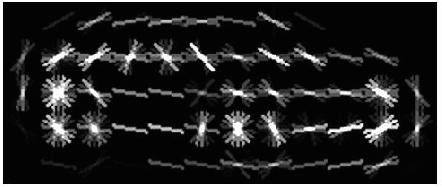
\includegraphics[width=\textwidth]{carhog_random}
                \caption{Initialised root filter after training against random negatives}
                \label{fig:carhog_random}
        \end{subfigure}
        \begin{subfigure}[b]{0.45\textwidth}
               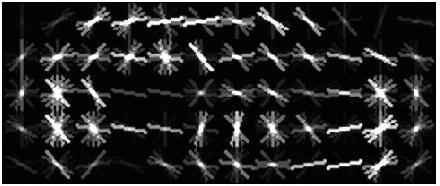
\includegraphics[width=\textwidth]{carhog_hard}
               \caption{Root filter after training against hard negatives}
                \label{fig:carhog_hard}
        \end{subfigure}
        \begin{subfigure}[b]{0.45\textwidth}
               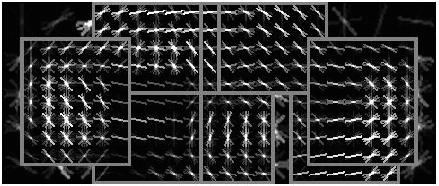
\includegraphics[width=\textwidth]{carhog_partinit}
               \caption{Mixture component after parts have been initialised}
                \label{fig:carhog_partinit}
        \end{subfigure}
        \begin{subfigure}[b]{0.45\textwidth}
               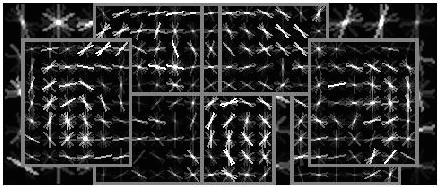
\includegraphics[width=\textwidth]{carhog_final}
               \caption{Mixture component after training against hard negatives}
                \label{fig:carhog_final}
        \end{subfigure}
\caption{This figure visualises the evolution of a mixture component of an eight viewpoint 3D DPM during the training procedure.}
\label{fig:carhog}
\end{center}
\end{figure}

\subsection{Initialisation}
An $n$-component model is initialised by first splitting the positive training examples according to aspect ratio statistics in $n$ training-sets,  and then training root filters for each component. Root filter dimensions are chosen in a way that their covered area is not greater than 80\% of the positive bounding boxes. Root filters are trained by warping positive bounding boxes to filter dimensions and training against negative examples obtained by extracting features from randomly selected regions of negative training images. Once all the root filters are initialised, the model is trained using several iterations of hard negative mining. Note that at this stage, only the component variable and root placement is treated as latent. 

The part filters are initialised by placing them on high "energy" regions, that is, regions with high euclidean norm of positive root filter weights. Possible part shapes are chosen from a pool of shape-templates and greedily added to the model. Regions covered by a part are zeroed out in the energy map and the next part is chosen until a fixed number of $k$ parts are added. In \cite{5255236} symmetry constraints on both the root and parts, are placed. Root filters are constrained to be symmetric along the vertical axis, as are parts lying on the centre vertical axis. Parts not lying in the centre have a symmetric partner.


\section{Extension to 3D}\label{sec:ext3D}
To extend the DPM to 3D, this project largely followed the approach of \cite{6248075} and \cite{Pepik:2012aa}. Training a 3D DPM relies highly on having viewpoint annotated training data. The model presented here is trained by using both real and synthetic training examples of cars. The synthetic examples were obtained by renderings of CAD models onto negative training images or backgrounds of mean pixel colour of the training images (see figure \ref{fig:CAD}). Experiments with both, orthographic and perspective projections for the rendering were done. Both \cite{6248075} and \cite{Pepik:2012aa} rely on rendered CAD models as well, but  they use non-photorealistic gradiant-based renderings and projective projections. For real training data, positive examples from the 3D object dataset \cite{4408987} and examples from VOC2012 \cite{pascal-voc-2012} with viewpoint annotations provided by \cite{xiang_wacv14} were used. 

\begin{figure}
\begin{center}
        \begin{subfigure}[b]{0.49\textwidth}
                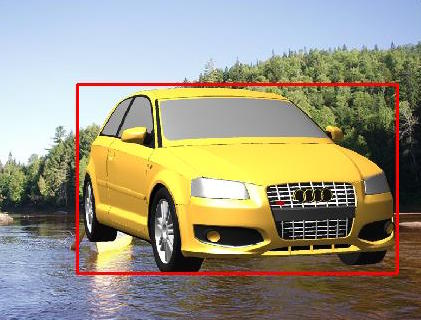
\includegraphics[width=\textwidth]{CADexample}
        \end{subfigure}
        \begin{subfigure}[b]{0.49\textwidth}
               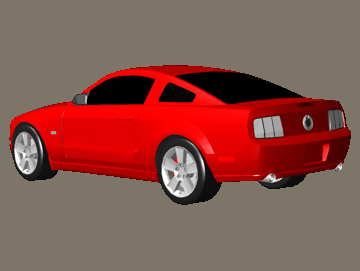
\includegraphics[width=\textwidth]{CADblack}
        \end{subfigure}
\caption{A CAD example rendered on a negative training image including the annotated bounding box (left). And a CAD example rendered on a background of mean pixels (right). Both were rendered using perspective projection.}
\label{fig:CAD}
\end{center}
\end{figure}

All the symmetry constraints placed on the root and parts from the original DPM \cite{5255236} were eliminated as they do not allow to distinguish different views (mirrored left and right side views of a car look identical). Figure \ref{fig:carhog} shows the evolution of one model view during the training procedure.


\subsection{Assigning Components to Viewpoints}
The first modification to the model was to relate mixture components to specific viewpoints. To achieve this, the training data $D$ was split according to viewpoint annotations into $n_c$ component training sets $\{D_i\}_{i=1}^{n_c}$ and root filters were initialised on each of these sets by training against random negatives (see figure \ref{fig:carhog_random}). Three parameters control the splitting of the training set: 
\begin{itemize}
  \item $n_c$: specifies the number of mixture components.
  \item $n_a$: specifies the number of different azimuth angles.
  \item $n_e$: specifies the number of different elevations. 
\end{itemize}
Note that $n_c=n_a\cdot n_e$. Viewpoints are split evenly across components, i.e. a model with $(n_c, n_a, n_e)=(16,8,2)$ would have eight azimuth angles lying in $\{0,45,90,135,180,225,270\}$. In this project a setting of $n_e=1$ was most often used while only varying $n_c$. Setting $n_e=2$ doubles the complexity of the model while only giving slight, if any, improvement in performance. Also, viewpoint accuracy as measured in  \cite{xiang_wacv14} only considers correct azimuth angle binning and example images from from VOC2012 \cite{pascal-voc-2012} typically don't vary much in elevation (see figure \ref{fig:hist}).

\begin{figure}
\begin{center}
        \begin{subfigure}[b]{0.49\textwidth}
                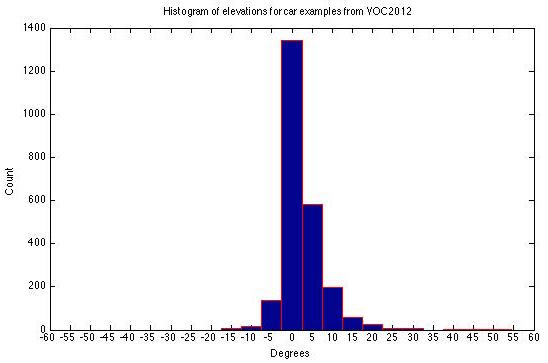
\includegraphics[width=\textwidth]{carElevHist}
        \end{subfigure}
        \begin{subfigure}[b]{0.49\textwidth}
                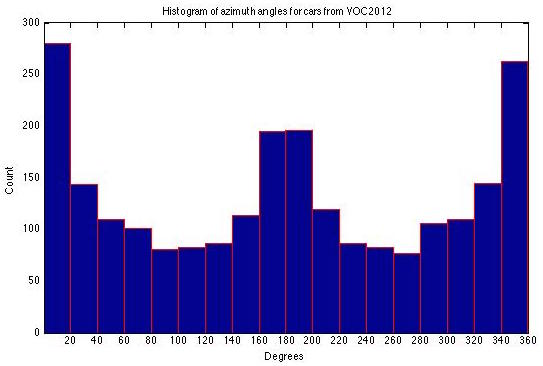
\includegraphics[width=\textwidth]{azimuthHist}
        \end{subfigure}
\caption{Histograms showing the distribution of elevations (left) and azimuth angles (right) across car examples from VOC2012 as annotated by \cite{xiang_wacv14}.}\label{fig:hist}
\end{center}
\end{figure}

During latent training, if a positive example falls within an angle $\Delta\alpha$ of a viewpoint assigned to a mixture component $c$, the latent component label is restricted to $c$. This has the nice side-effect of speeding up training as we do not have to search over all the components. Choosing $\Delta\alpha$ leads to a trade-off between precision and viewpoint accuracy. A value of $\Delta\alpha\in[10,...,20]$ was found to perform well. 

Another way of enforcing the correct component label during training is to introduce a penalty for incorrect viewpoint predictions. Formally, the labels of positive examples are extended by a component label $y_c$ leading to $y=(y_l,y_b,y_c)$. During latent positive search, latent variables would then be set to:
\begin{equation}\label{eq:penalty}
 z'=\argmax_{z\in Z(x,y)}(\beta\cdot\Phi(x,z)-l(y_c,c))
\end{equation}
where $l(y_c,c)=\mathbbm{1}{ [y_c\neq c] *\gamma}$ is the penalty term and the parameter $\gamma$ controls the weight of correct viewpoint assignments. The value of $\gamma$ was set to $\gamma=\max(1,\beta\cdot\Phi(x,z)/2)$. This way, very confident hypotheses are penalised more if they lead to wrong viewpoint estimates.  Experiments showed that this generally doesn't decrease detection performance while increasing viewpoint accuracy. 

\subsection{Placing Parts in 3D}
Going from 2D to 3D, anchor positions should now be placed in 3D object space rather than in the 2D root filter. As a reference coordinate system, a 3D object box is created and the origin is placed at the centre of the 3D box (see section \ref{sec:partInit} for details). Analogous to \cite{6248075}, parts are parametrised by part boxes $b_i=(s_{x_i},s_{y_i},s_{z_i})$ co-aligned with the object box. The new anchor position $v_i=(x_i,y_i,z_i)$, now in 3D, specifies the center of the part box in object coordinates. 

Part filters remain 2D templates of weight vectors and are sized so that they tightly cover the 3D part box as seen from the viewpoint of each mixture component. Mapping the 3D anchor positions to root filter coordinates is done by using an orthographic projection $P_c$ given by the viewpoint of component $c$. 

To make sure that part filters are learned consistently across views, latent part positions have to be inferred in 3D and simultaneous for all views of a given car model. This is achieved by making use of the CAD training data. Concretely, positive CAD examples are labeled with a model-ID $y_o$ and  a set $D(i)=\{(x,y)\in D:y_o=i\}$ is created. As CAD examples come with perfect annotations, the root placement and component variable are fixed. The root placement $p_c$ of component $c$ is chosen such that it yields maximum overlap with the annotated bounding box $y_b$. An object hypothesis in 3D is now defined by $h=(q_1,\ldots,q_n)$ where $q_i=(x_i,y_i,z_i)$ specifies the position of part $i$ in object coordinates. Note that for model component $c$ we get $z=(c,p_c,P_c(q_1),\ldots,P_c(q_n))$, the connection to the 2D hypothesis. Parts are still fixed to be an octave below the root filter in the feature pyramid. Let $\Psi(x,y,h)=\Phi(x,z(y,h))$, where $z(y,h)=(y_c,p_c,P_c(q_1),\ldots,P_c(q_n))$. The objective is now to find:
\begin{equation}\label{eq:3dConstraints}
	h'=\argmax_{h}(\sum_{(x,y)\in D(i)}\beta\cdot\Psi(x,y,h))
\end{equation}
Note that part displacements are still modelled in 2D (as in the model of \cite{6248075}) and are only dependent on other views via equation \ref{eq:3dConstraints}. This is in contrast to \cite{Pepik:2012aa} where displacements are modelled in 3D. While the 3D deformation model increases the models performance on ultra-wide baseline matching experiments, performance decreased for both detection and viewpoint estimation.

For each car model $i$ the procedure to solve \ref{eq:3dConstraints} is the following:
\begin{description}
  \item[1. Step]  Construct a 3D grid of possible part placements by padding the 3D object box to all sides. Padding is used to allow parts to move out of the 3D object box. 
  \item[2. Step] Compute feature maps for root and part filters for all examples $(x,y)\in D(i)$. The feature maps are computed so that they cover the whole 3D grid as seen from viewpoint $y_c$ and the fixed root placement yields maximum bounding box overlap.
  \item[3. Step] Iterate each part $p_j$ through each position $q_i$ of the 3D grid and sum up the scores for placing part $p_j$ at position $q_i$ for all the views. For a view related to component $c$, the score is given by  the score of placing it at $P_c(q_i)=(x_i,y_i)$ in root filter coordinates. That is, $score(p_j,q_i,c)=F'_j\cdot \phi(H,P_c(q_i))-d_j\cdot \phi_d (dx_j,dy_j)$. Note that here $H$ denotes the feature maps computed in step 2 and not a feature pyramid as in section \ref{sec:defParts}. The total score for placing $p_j$ at $q_i$ is then given by $score(p_j,q_i)=\sum_cscore(p_j,q_i,c)$.
  \item[4. Step] Pick the position that yields the highest overall score for each part. We set $h'=(\argmax_{q}score(p_1,q),\ldots,\argmax_{q}score(p_n,q))$.
\end{description}

Positive training examples for which no model-ID is provided, are treated as before, i.e. projecting the 3D anchor position to 2D and then searching for the best hypothesis in 2D. 

\subsection{Initialising Parts in 3D}\label{sec:partInit}

The initialisation of parts in 3D follows a similar heuristic as the 2D DPM by greedily placing them on high energy regions in 3D. For initialising a model with $m$ parts, the procedure is the following:  \begin{description}
  \item[1. Step] First the 3D object box is created which will be used to set up a grid of possible part placements. The box is modelled as 3D array of zeros. The dimensions of the box are initialised from the dimension of front and right view root filters. The height is set to twice the height of the front filter. The front and right view dimensions are then warped to fit the height of the box while preserving the aspect ratios. 
  \item[2. Step] Next, a pool of possible 3D part boxes $b_i=(s_{x_i},s_{y_i},s_{z_i})$ is created. Each part box is sized so that its volume approximately covers $1/m$ of the object box volume, concretely: $V_{part}=0.8*\frac{V_{object}}{m}$. 
  \item[3. Step] Each part box is then convolved with the 3D object box to get a grid of possible part placements. The part box is then moved through the grid and each grid position is assigned an energy. The energy of a grid position $q=(x,y,c)$ is obtained by projecting $q$ onto the root filters of all the components and then summing up the norm of positive root filter weights covered by the part box for all the components.
  \item[4. Step] The highest scoring shape and position combination is then chosen as new 3D part. To get non overlapping parts, regions covered by the new part are set to $-100$ in the 3D object box. This way, convolving the object box with the part shapes in step 3 gives grid positions that lead to overlapping parts a negative energy.
  \item[Repeat Step 3 and 4 until $m$ parts are chosen] 
\end{description}

As not all of the 3D parts are visible from all the views, only a maximum of $k$ parts are assigned to each view. For each view, parts are chosen greedily based on both their energy on the root filter and their depth in the 3D object box as seen from this view (parts in front are preferred). When a 3D part gets chosen, the region it covers is zeroed out in the root filter energy and a next part is chosen until either all $k$ parts are chosen or no more regions of the root energy can be covered by other parts (Note that different components might now have a different number of parts assigned to them). Part filters are chosen such that they tightly cover the 3D part box as seen from that view (see figure \ref{fig:3dbox}).

\begin{figure}
\begin{center}
           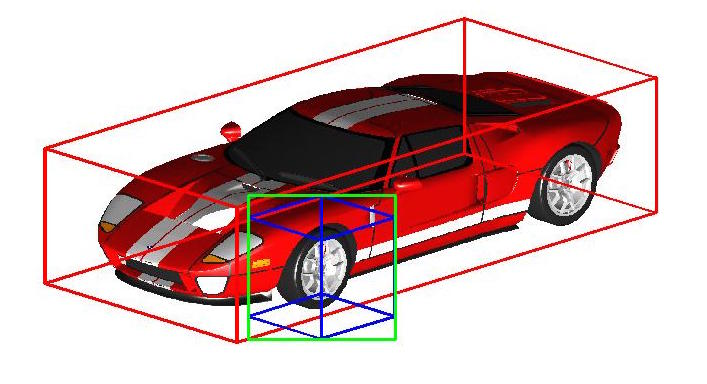
\includegraphics[width=0.8\textwidth]{3dbox}
\caption{This figure illustrates the idea of the 3D object box and the part parametrisation. The blue box represents a 3D part box and the green 2D box represents the part filter template from the given viewpoint.}
\label{fig:3dbox}
\end{center}
\end{figure}


\section{CNN Features}\label{sec:cnnFeat}
This section covers the steps taken to replace the HOG features of the original DPM with CNN features. The features used in this project are computed using the MatConvNet toolbox \cite{arXiv:1412.4564}. The concrete net used was the fast CNN-F architecture described in \cite{Chatfield14}. The net consists of 5 convolutional layers, some of which are followed by max-pooling layers, and 3 fully connected layers. The architecture used is similar to the one by Krizhevsky et al. \cite{krizhevsky2012imagenet} with the difference of having dense connectivity between convolutional layers in CNN-F and less convolution kernels in layers 1 (64 vs.96) and layers 3 and 4 (256 vs 384 each).

The standard input of CNN-F is a fixed sized $224\times224\times3$ image patch which is preprocessed by subtracting the mean training image. Constructing the feature pyramid requires to compute features for several rescaled versions of images of variable size. This project therefore used arbitrarily sized images as input to the CNN and approximated the normalisation by subtracting the mean pixel value from the input image. This approach was also used and experimentally justified in \cite{DBLP:journals/corr/IandolaMKGDK14} on the Caffe net \cite{jia2014caffe}. CAD examples were rendered on a background of the same mean pixels (see figure \ref{fig:CAD} right). 

Only the first five convolutional layers of the network are used to compute features (also discarding the last max-pooling layer). The output of the fifth convolutional layer given an input image of size $224\times224\times3$ is a feature map of size $13\times13\times256$. To get a more convenient mapping from image coordinates to feature map, the inputs of all the convolutional and max-pooling layers with kernel size $k$ are padded by $\lfloor k/2\rfloor$ with zeros to all sides (see table \ref{tab:cnn}). The output of a $224\times224\times3$ is then a $14\times14\times256$ feature map and coordinates $(x,y)$ in the feature map, map to $(16x,16y)$ in image coordinates (16 is the stride of the features computed by the fifth convolutional layer). For HOG features, the mapping was given by $(8x,8y)$ where 8 is the HOG cell size. This approach is similar to the one of \cite{girshick2014deformable} and was found to work slightly better than simply padding the feature maps to obtain the same mapping (used in \cite{DBLP:journals/corr/IandolaMKGDK14} and \cite{savalle8deformable}).

\begin{table}
\begin{center}
\begin{tabular}{|c||c|c|c|c|c|c|c|}
\hline
Layer & conv$_1$ & pool$_1$ &  conv$_2$ & pool$_2$ & conv$_3$ & conv$_4$ & conv$_5$ \\
\hline \hline
\#Filters & 64 & - & 256 & -& 256 &  256 &  256 \\
\hline
Size	& $11\times11$ & $3\times3$ & $5\times5$ & $3\times3$ &  $3\times3$ &  $3\times3$ &  $3\times3$  \\
\hline
Stride & 4 & 2 & 1 & 2 & 1 & 1 & 1\\ 
\hline
Padding & 5 & 1 & 2 & 1 & 1 & 1 & 1\\
\hline
\end{tabular}
\caption{This table shows the architecture of the first five layers of  the CNN-F network with the modified padding.}
\label{tab:cnn}
\end{center}
\end{table}

The feature vectors obtained by the fifth convolutional layer are further standardised, i.e. the mean feature vector is subtracted and an element-wise division by the standard deviation of the feature vectors is performed. This has shown to be very important for the SVM training (see section \ref{sec:cnnexp}). Also, it was found  to be important to adjust the SVM parameter C for CNN features. While HOG features work well with a value of $C=2\cdot10^{-3}$, a value of $C=2\cdot10^{-5}$ was found to work better with CNN features. This lower value of $C$ places more focus on maximising the margin of the classifier and reduces the risk of overfitting to the training data.

By observing the detections during latent positive search, another necessary adjustment to the models parameters became apparent. The quadratic deformation parameters of HOG based DPMs are lower bounded by a value of $0.01$ ensuring that the deformation model doesn't become too "flat". This lower bound showed to be too low for CNN features however, as the parts tend to move away very far from their anchor positions (sometimes placed on other cars in the scene) and also hindered the convergence of the hard negative training. This can be explained by the lower influence the deformation features/parameters have on the overall score of a hypothesis. The lower bound was therefore raised to $0.2$, which fixed the issues.

Switching from HOG to CNN features brings four significant changes: 

\begin{enumerate}
\item
The subsampling factor from image to feature map is doubled from 8 to 16. If the root filter dimensions are kept unchanged, this implies that the smallest objects that can be detected by a CNN-DPM are twice as large as the smallest detectable objects for a HOG-DPM. To counteract this, the oversample factor of the first level of the feature pyramid is increased from 2 to 4, which makes the feature pyramids equivalent with respect to the root filter sizes (doubled root and feature map sizes).
\item
HOG features describe scale invariant local gradient statistics while CNN features describe large, highly overlapping  $163\times163$ image patches. This might be one reason why it is beneficial to use poorly localised positive examples as negative training examples as reported by \cite{girshick2014deformable} and \cite{girshick2013rich}. Poorly localised in this case means examples that lead to a ground truth bounding box overlap of less than $0.3$.  
\item
The feature vector dimension increases from 31 to 256. This of course slows down training significantly as well as increases the time needed to compute the convolutions of the model filters with the feature maps during inference considerably. One possibility to counteract the slower training would be to employ the Linear Discriminative Analysis (LDA) based acceleration to DPM training \cite{girshick2013training}. In this project however, the SVM training procedure has been preserved (allowing a better comparison to HOG features) and training iterations have been reduced as CNN models have been found to converge faster. 
\item
The feature computation takes much longer on a CPU. This makes the computation of the feature pyramid  considerably slower, typically increasing the computation time by a factor of four. In this project therefore the number of levels per pyramid ($\lambda$) was reduced from five to two during training, sacrificing some performance in favour of faster training and inference. \cite{girshick2014deformable} reported that this modification still provided good enough feature  localisation and experiments conducted in this project also found that increasing $\lambda$ for CNN features only slightly increases performance. This of course also speeds up inference as much less convolutions are needed.
\end{enumerate}


\section{Performance Optimisation}
As the model presented here is based on DPM VOC-release 3, there is an inherent performance gap to newer versions (e.g. DPMver4 \cite{voc-release4} or DPMver5 \cite{voc-release5}). To close this gap, several improvements introduced in DPMver4 have been adopted to the model described here. 

To speed up training:
\begin{itemize}
  \item Positive and hard negative search has been implemented in parallel, and convergence criteria were added. Training stops if relabelling doesn't reduce positive loss by much and hard negative mining stops and skips to the next latent positive search if the negative loss on the full negative training set doesn't increase the negative loss by much.
  \item The C++ training code has been updated to the one used in DPMver4. It features better learning statistics and adds convergence criteria. A new stopping criteria, where training stops if the sum of positive and negative loss  don't exceed a certain value $\epsilon$, has also been added. This is only affecting the CNN training however, and should also prevent overfitting to a certain degree.
  \item For viewpoint annotated data with viewpoints inside a range of $\alpha$ of a model's viewpoint angle, latent positive search has been restricted to examples with the correct component label.
\end{itemize}

Section \ref{sec:expparam} gives an experimental evaluation of several model parameters and design choices on the models detection and pose-estimation performance. Two of the most significant performance boosts come from adding an extra octave to the feature pyramid and the use of a truncation feature.

\begin{figure}
\begin{center}
        \begin{subfigure}[b]{0.5\textwidth}
                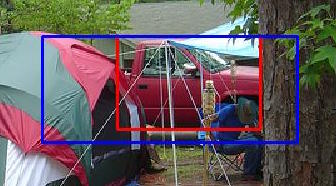
\includegraphics[width=\textwidth]{occluded}
        \end{subfigure}
        \begin{subfigure}[b]{0.4\textwidth}
                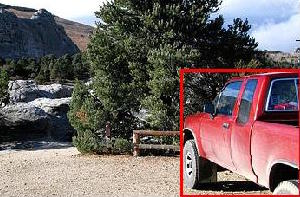
\includegraphics[width=\textwidth]{truncated}
        \end{subfigure}
\caption{Figures illustrating problems with the bounding box annotations on Pascal VOC. The red bounding boxes are the annotations and the blue bounding box illustrates the discrepancy to a real car bounding box.}
\label{fig:trunc}
\end{center}
\end{figure}

\subsection{Handling Truncated and Occluded Objects}\label{sec:trunc}

In experiments on the Pascal VOC 2012 dataset which contains several truncated and occluded objects, the importance of handling truncated and occluded objects effectively became apparent (see figure \ref{fig:trunc}). In this project two approaches were tested to improve  detection of truncated objects.

To detect truncated objects, all levels of the feature pyramid are padded with zeros by half the root size. In DPMver3 the computation of the bounding box overlap requirement during latent search (0.7 overlap) is computed using the root filter box. This discards a lot of truncated examples or leads to wrong component labels as the correct root placement is prohibited by the overlap requirement. An easy fix for this is to clip the root box of truncated examples to image boundaries before computing the overlap. 
It showed that detection performance can be improved further by padding the feature pyramid with the mean hog features computed on positive training examples. An even better performing approach is to augment the feature vectors with an additional truncation bias term  (used in \cite{voc-release4}). This feature term is set to 0 if the feature vector is placed within image boundaries and to 1 if it is outside the image boundaries. This way, the model actually learns which filter regions often are truncated. 

Another observation made on occluded examples was that the minimum bounding box overlap requirement  of 0.7 during latent positive search would often prohibit the correct viewpoint from being chosen. For occluded examples (indicated through annotation) the minimum bounding box requirement was therefore reduced to 0.5.  
As un-occluded and non-truncated object instances should be expected to have "good" bounding boxes in the sense that the model's detection should lead to high bounding box overlap, the penalty term from equation \ref{eq:penalty} has been extended with an overlap penalty term leading to:
\begin{equation}
l(y,z)=(0.5\cdot\mathbbm{1}{ [y_c\neq c] }+0.5\cdot \frac{A_z\cap A_y}{A_z\cup A_y})*\gamma
\end{equation}
Where $A_z$ is the area covered by the hypothesised root filter placement and $A_y$ is the area covered by the annotated bounding box. The intuition behind this was that this enforcing of good bounding box localisation has a similar positive effect as the structured output formulation of \cite{6248075}, while being more flexible as the bounding box overlap is only penalised if the object is in full sight. 

\chapter{Experiments and Results}\label{chap:exp}

\section{Influence of Model Parameters}\label{sec:expparam}
This section presents experimental results concerning the influence of several model parameters. The model presented in this work has a variety of different parameters that can have an influence on its performance. These parameters concern:
\begin{description}
\item[Training data:] \hfill 
\begin{itemize}
\item The amount of training data
\item Synthetic vs. real vs. mixed data
\item Orthographic vs. perspective CAD rendering
\item Backgrounds of rendered CAD examples (negative examples vs. mean pixels)
\item Angle $\alpha$ for which an example's viewpoint is fixed during training
\end{itemize}
\end{description}

\begin{description}
\item[Model:] \hfill 
\begin{itemize}
\item Number of views/mixture components
\item Number of 3D parts
\item Number of visible parts per viewpoint
\item Rootfilter dimension/area
\item Number of elevations the model is trained on
\end{itemize}
\end{description}

\begin{description}
\item[Learning:] \hfill 
\begin{itemize}
\item L-SVM parameters C and J (cost weighting factor for positive examples)
\item Influence of incorrect viewpoint penalty
\end{itemize}
\end{description}

\begin{description}
\item[Features:] \hfill 
\begin{itemize}
\item HOG vs. CNN
\item Truncation feature
\item Standardisation of CNN features
\item Extra octave for feature pyramid
\end{itemize}
\end{description}

To test the influence of some of these parameters and maximise performance of the model, experiments were conducted on the VOC 2012 validation data. For most of the experiments, all but one parameter were kept fixed and a model was trained with different values for the given parameter. After evaluating the performance of the model on the validation set, the best performing parameter value was chosen and fixed during experiments with other parameters.  Both average precision as measured by the VOC criteria (a minimum of 0.5 bounding box overlap) and viewpoint accuracy (0.5 overlap and correct viewpoint) proposed by \cite{xiang_wacv14} were used as performance measures. Tables \ref{tab:modelParam}-\ref{tab:otherParam} show the results for some parameters as relative performance loss or gain for different values. 

%
\begin{table}[]
	\parbox{.45\linewidth}{
		\centering
		\begin{tabular}{|c|c|c|}
		\hline
		 Root Area & AP & VA \\
		\hline\hline
		 57-67 & 0 & 0  \\
		\hline 
		 62-72 & +1.1 & +1.4 \\
		\hline
		 67-77 & +0.4 & +0.2 \\
		\hline
		\end{tabular}
		\subcaption{Relative AP and VA for different root area constraints (min-max)}
		\label{tab:rootarea}
	}		
	%
	\parbox{.45\linewidth}{
		\centering
		\begin{tabular}{|c|c|c|}
		\hline
		 \#Components & AP & VA\\
		\hline\hline
		 4 & 0 & 0\\
		\hline 
		 8  & +1.2 & +0.6 \\
		 \hline 
		 16 & -0.7 & -6.2\\
		 \hline
		\end{tabular}
		\subcaption{Relative AP and VA for different numbers of mixture components}
		\label{tab:numComp}
	}		
	%
	\parbox{\linewidth}{
		\centering
		\begin{tabular}{|c|c|c|c|}
		\hline
		 \#3D parts & Max parts per view & AP & VA\\
		\hline\hline
		 12 & 8 & 0  & 0\\
		\hline 
		 16 & 10 & +0.4 & -0.3\\
		 \hline 
		 20 & 12 & +1.2 & +0.8\\
		 \hline
		\end{tabular}
		\subcaption{Relative AP and VA for different numbers of 3D-parts and parts per view (PpV)}
		\label{tab:parts}
	}	
	%
	\parbox{.5\linewidth}{
		\centering
		\begin{tabular}{|c|c|c|c|}
		\hline
		 \#elevations & AP & VA\\
		\hline\hline
		 1 & 0  & 0\\
		\hline 
		 2 & -0.9 & -0.6\\
		 \hline 
		\end{tabular}
		\subcaption{Relative AP and VA for different numbers of elevations}
		\label{tab:elev}
	}
	%
	\parbox{.5\linewidth}{
		\centering
		\begin{tabular}{|c|c|c|c|}
		\hline
		 Extra pyramid octave & AP & VA\\
		\hline\hline
		 without & 0  & 0\\
		\hline 
		 with & +5.2 & +3.1\\
		 \hline 
		\end{tabular}
		\subcaption{Relative AP and VA for models with or without an extra pyramid octave}
		\label{tab:extraoctave}
	}
	\caption{Tables showing the influence of several model parameters on average precision (AP) and average viewpoint accuracy (VA).}
	\label{tab:modelParam}
\end{table}
%
Table \ref{tab:rootarea} illustrates the influence of the constraints on the model's root filter areas in feature dimensions. We can observe that the performance decreases for areas of sizes between 57 and 67 or 67 and 77 compared to  root filter areas  of sizes between  62 and 72. Smaller root areas lead to filters that do not capture enough detail and therefore might miss some meaningful details of the object's appearance. As root filter areas have a direct influence on the size of the smallest perceivable object instances, bigger root filters lead to fewer detections of small objects. 

The influence of the number of mixture-components/views can be observed in table \ref{tab:numComp}. Note that viewpoint accuracy (VA) decreases significantly when increasing number of views from 8 to 16. This is expected as more views lead to a finer binning of viewpoints and neighbouring viewpoints therefore get more difficult to discriminate. We can also observe that detection performance increases when going from 4 views to  8. This can be explained by a more complex model and an increased variety of aspect ratios covered by the root filters. The slight decrease in performance when going from 8 views to 16 could be explained by the fact that more model components result in a reduction of training examples for each component. 

The influence of different amounts of parts can be seen in table \ref{tab:parts}. We see that increasing the number of parts generally increases the performance of the model. Note that by construction (section \ref{sec:partInit}) more 3D parts lead to smaller 2D part-templates. Also, the model's complexity doesn't increase by much  as part filters are only added until no more root filter area can be covered by new parts. Therefore the model effectively just grows from the additional deformation parameters. 

Surprisingly, training models on more than one elevation didn't lead to better performance (table \ref{tab:elev}). A possible explanation for this observation could be found in the distribution of object viewpoints in the data sets (see figure \ref{fig:hist}). As there are not many examples having an increased elevation there are not a lot of training examples for the new components and the training data of the more important (ground-level) views is reduced.

One of the most significant boosts in performance was observed when training the model with an extra octave added to the feature  pyramid (table \ref{tab:extraoctave}). The highest resolution feature maps computed on an extra octave pyramid are computed at four times the resolution of the original image. This modification leads to more training examples, as some examples were just too small to be used with the normal pyramid, and also allows the model to detect smaller object instances at test time. It should be noted however that this performance gain come at the cost of increased detection and training time. 

\begin{table}[]
	\parbox{.45\linewidth}{
		\centering
		\begin{tabular}{|c|c|c|}
		\hline
		Training data & AP & VA\\
		\hline\hline
		 Real only & 0 & 0\\
		\hline 
		 Real+CAD persp. & -1 & -0.6 \\
		 \hline 
		 Real+CAD ortho. & -1.9 & -2\\
		 \hline
		\end{tabular}
		\subcaption{Relative AP and VA for different training data}
		\label{tab:data}
	}		
	%
	\parbox{.45\linewidth}{
		\centering
		\begin{tabular}{|c|c|c|}
		\hline
		Fixation angle $\alpha$ & AP & VA\\
		\hline\hline
		 20 & 0 & 0\\
		\hline 
		 45  & -1 & +0.2 \\
		 \hline 
		 5 & -0.5 & -0.4 \\
		 \hline
		\end{tabular}
		\subcaption{Relative AP and VA for different viewpoint fixation angles.}
		\label{tab:alpha}
	}	
	\parbox{\linewidth}{
		\centering
		\begin{tabular}{|c|c|c|}
		\hline
		CAD background& AP & VA\\
		\hline\hline
		 Negative training images & 0 & 0\\
		\hline 
		 Mean pixels of CNN features & +0.8 & +2.3 \\
		 \hline 
		\end{tabular}
		\subcaption{Relative AP and VA for different backgrounds of the CAD training examples}
		\label{tab:background}
	}
	\caption{Tables showing the influence of training data parameters.}
	\label{tab:dataParam}
\end{table}

In table \ref{tab:data} we can observe the influence of different training data configurations. Note that training a model on only real training data implies that no 3D-constraints can be enforced on the model and parts are learnt fully independent across views. This can be one explanation why there is an improvement in performance compared to training on a combination of synthetic and real images, as parts can be learnt optimally for each separate view. Also, the importance of using perspective projections for rendering becomes apparent. While orthographic projections are a reasonable approximation for far away objects, real images of cars often are taken from a rather close distance. As table \ref{tab:background} shows, uniform backgrounds showed to work better than backgrounds of negative training images.  

The influence of the angle $\alpha$ which defines the range of viewpoints that are going to be assigned to a fixed mixture component during training is shown in table \ref{tab:alpha}. The choices for $\alpha$ here are listed for a four-component-model and of course $\alpha=min(\alpha,360/(2*\#Comp))$ holds. As expected a value of $\alpha=45$, which means in this case that all examples are fixed to their correct viewpoint, increases viewpoint accuracy but decreases detection performance significantly. More surprising is that an angle of 5 decreases performance in both tasks compared to an angle of 20. 

\begin{table}[]
	\parbox{.45\linewidth}{
		\centering
		\begin{tabular}{|c|c|c|}
		\hline
		Penalty term $l$ & AP & VA\\
		\hline\hline
		 without & 0 & 0\\
		\hline 
		 with & +0.5 & +2.8 \\
		 \hline 
		\end{tabular}
		\subcaption{Relative AP and VA influence of penalty term.}
		\label{tab:penalty}
	}	
	%	
	\parbox{.45\linewidth}{
		\centering
		\begin{tabular}{|c|c|c|}
		\hline
		Truncation feature & AP & VA\\
		\hline\hline
		 without & 0 & 0\\
		\hline 
		 with & +7.9 & +7.5 \\
		 \hline 
		\end{tabular}
		\subcaption{Relative AP and VA influence of penalty term.}
		\label{tab:truncfeat}
	}		
	\caption{Tables showing the influence of penalty term and truncation feature.}
	\label{tab:otherParam}
\end{table}

As we can see from table \ref{tab:penalty} the penalty term $l$, introduced to softly enforce the correct viewpoints (equation \ref{eq:penalty}), does not only deliver a better viewpoint-estimation performance but also slightly raises detection performance. Again, we observe that correct viewpoint assignments favour the detection performance. Table \ref{tab:truncfeat} shows the significant performance boost obtained by the truncation feature and the related adjustments described in section \ref{sec:trunc}.

\begin{table}[]
\resizebox{0.7\linewidth}{!}{\begin{minipage}{\textwidth}
	\begin{center}
		\begin{tabular}{|c|c|c|c|c|c|c|}
		\hline
		 3D-DPM & 3D-DPM+ & DPMver3 \cite{5255236} & DPMver4 \cite{voc-release4} & DPM-VOC \cite{6248075} & DPM 3D-Const. \cite{6248075} & 3D2PM \cite{Pepik:2012aa}\\
		\hline\hline
		53.9 & 63.4 & 50.2 & 57.9 & 66 & 63.1 & 61.2\\
		\hline
		\end{tabular}
	\end{center}
\end{minipage} }
\caption{Average Precision (AP) on cars of the VOC 2007 \cite{pascal-voc-2007} test set. Results for the model in this project are given in the first two columns and results of other models are provided for comparison.}\label{tab:voc2007}
\end{table}

%\begin{table}[]
%\resizebox{\linewidth}{!}{\begin{minipage}{\textwidth}
%	\begin{center}
%		\begin{tabular}{|c|c|c|c|}
%		\hline
%		3D-DPM & DPM & DPM 3D-Const. & 3D2PM\\
%		\hline\hline
%		63.4 & 57.9 & 63.1 & 61.2\\
%		\hline
%		\end{tabular}
%	\end{center}
%\end{minipage} }
%\caption{Average Precision (AP) on cars of the VOC 2007 \cite{pascal-voc-2007} test set. Results for the model in this project are given in the first two columns and results of other models are provided for comparison.}\label{tab:voc2007}
%\end{table}

\section{Bounding Box Localisation}\label{sec:boxloc}
To test the model's detection performance the model was evaluated on the well known and challenging Pascal VOC 2007 \cite{pascal-voc-2007} dataset, the VOC 2012 \cite{pascal-voc-2012} 'val' set, and the 3D object dataset \cite{4408987}.   The performance measure used is the standard VOC measure of a minimum ground truth bounding box overlap of 50\%.

Table \ref{tab:voc2007} reports the results on VOC 2007 of the model implemented in this project (3D-DPM and 3D-DPM+) and also lists results for different versions of the DPM and similar models. 3D-DPM is an eight-view-model  which was trained on perspective CAD examples and real training images from VOC 2007 'trainval'. 3D-DPM+ was trained on additional training data from VOC2012 'train', the first five car models of 3D object dataset and uses an extra octave pyramid. 

We see that the 3D-DPM outperforms DPMver3 on which it is built upon and doesn't quite perform as good as DPMver4. The performance improvements with respect to DPMver3 can largely be attributed to the addition of the truncation feature, as well as the higher number of components. A possible explanation for the performance difference to DPMver4 could lie in the fact that VOC 2007 examples come without viewpoint annotations and therefore the model is initialised on CAD examples only (which might lead to sub-optimal filter dimensions and initialisations). Using additional examples from VOC 2012 in fact showed to increase the performance to around the same value as DPMver4 achieves. Another explanation can be found in the 3D constraints, which have already showed to have a negative impact on detection performance.

Compared to the other 3D DPM implementations DPM 3D-Constraints \cite{6248075} and 3D2PM \cite{Pepik:2012aa}, 3D-DPM performs worse. On the other hand, the performance boost of 3D-DPM+ obtained by the use of an extra pyramid octave lifts its performance above the ones reported for the other two 3D models \cite{Pepik:2012aa} \cite{6248075}. This suggests that these models most probably also made use of an extra octave pyramid, an implementation detail not mentioned in their publications. As \cite{6248075} report an average precision of 63.3 on VOC 2007 cars without the SSVM formulation and without the addition of synthetic training data, no other design choice seems to justify the performance difference to 3D-DPM or DPMver4. 

\begin{table}[]
\resizebox{1\linewidth}{!}{\begin{minipage}{\textwidth}
	\begin{center}
		\begin{tabular}{|c|c|c|c|c|}
		\hline
		\#views & 3D-DPM & 3D-DPM+ & VDPM \cite{xiang_wacv14} & DPM-VOC+VP \cite{6248075}\\
		\hline\hline
		4 &  38.2/30.2 & 47.4/37.3 & 37.2/20.2 & 45.6/36.9\\
		\hline
		8 &  39.4/30.8 & 49.4/35.5 & 37.3/23.5 & 47.6/36.6\\
		\hline
		16 & 37.5/24.0 & 47.5/29.5 & 36.6/18.1 & 46.0/29.6\\
		\hline
		\end{tabular}
	\end{center}
\end{minipage} }
\caption{Average precision and average viewpoint accuracy (AP/VA) on cars of the VOC 2012 'val' set with annotations by \cite{xiang_wacv14}.}\label{tab:voc2012}
\end{table}

Table \ref{tab:voc2012} lists the AP of 3D-DPM and 3D-DPM+ on the VOC2012 'val' dataset. It also shows results for DPM-VOC+VP \cite{Pepik:2012aa} and VDPM which is a modification of DPMver4 in which root filters are initialised on training sets that are obtained by binning the annotated VOC2012 test data of \cite{xiang_wacv14} into $k$ viewpoint bins. After the initialisation on the correct viewpoints, training is identical to the standard DPM training of DPMver4. Here, we observe that 3D-DPM achieves consistently higher average precision compared to VDPM (DPMver4) and considerably worse than DPM-VOC+VP. On the other hand, 3D-DPM+ achieves the highest average precision of all the listed models. Some of the performance gain compared to DPM-VOC+VP might be due to the higher amount of training data.

\begin{table}[]
\resizebox{0.9\linewidth}{!}{\begin{minipage}{\textwidth}
	\begin{center}
		\begin{tabular}{|c|c|c|c|c|}
		\hline
		3D-DPM & 3D-DPM+ & DPM 3D-Const. \cite{6248075} & 3D2PM \cite{Pepik:2012aa} & DPM-VOC+VP \cite{6248075}\\
		\hline\hline
		99.1/96.7 & 98.2/93.3 & 99.7/96.3 & 99.6/95.8 & 99.9/97.9\\
		\hline
		\end{tabular}
	\end{center}
\end{minipage} }
\caption{Average precision and viewpoint estimation in MPPE on cars of the 3D Object classes dataset \cite{4408987}.}	\label{tab:3DDataset}
\end{table}

Finally, the results on the 3D object classes dataset \cite{4408987} are shown in table \ref{tab:3DDataset}. This is a rather easy dataset as all the cars are in full sight and the viewpoints exactly match the viewpoints an eight-view-model is trained on. For comparison the results for other models are listed as well. Note however, that for these models it is unclear which of the examples in the dataset were used for testing. While they state that a subset of the examples was used for training, the exact assembly and size of the subset is unknown, making the comparison difficult. 3D-DPM is trained on CAD renderings, examples from VOC2012 and the first five (of ten) car models of the 3D object dataset. The last five car models were used for testing. It is interesting to notice that 3D-DPM+ performs slightly worse than 3D-DPM on this occasion. As the dataset is also relatively small (only 480 car examples in total), these performance differences should be taken with a grain of salt. Overall, the performance is comparable to the other models.

%\begin{figure}
%\begin{center}
%        \begin{subfigure}[b]{0.49\textwidth}
%                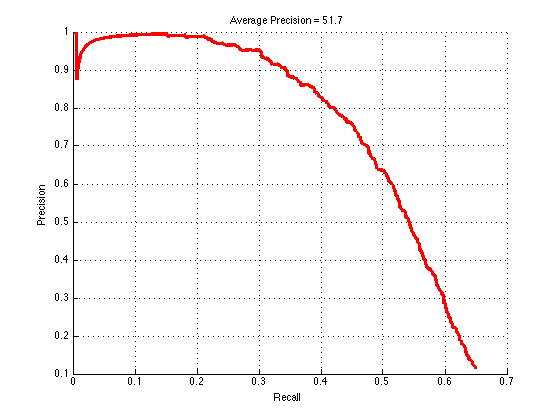
\includegraphics[width=\textwidth]{voc20074comp}
%               	\caption{VOC 2007 4 views}
%        \end{subfigure}
%        \begin{subfigure}[b]{0.49\textwidth}
%                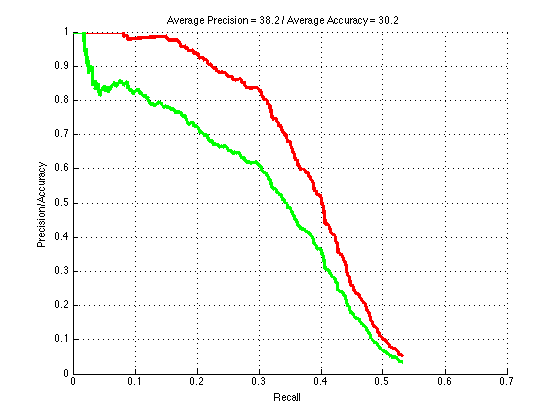
\includegraphics[width=\textwidth]{voc20124comp}
%                \caption{VOC2012 4 views}
%        \end{subfigure}
%        \begin{subfigure}[b]{0.49\textwidth}
%                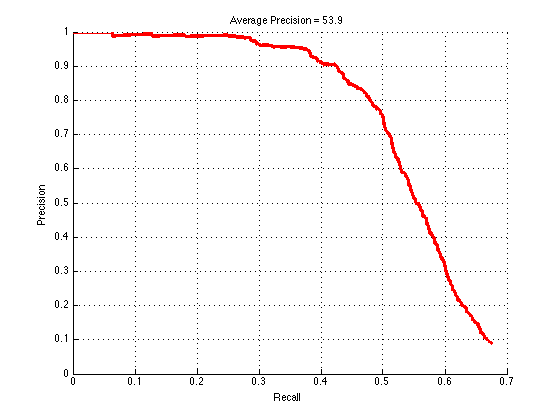
\includegraphics[width=\textwidth]{voc20078comp}
%               	\caption{VOC 2007 8 views}
%        \end{subfigure}
%        \begin{subfigure}[b]{0.49\textwidth}
%                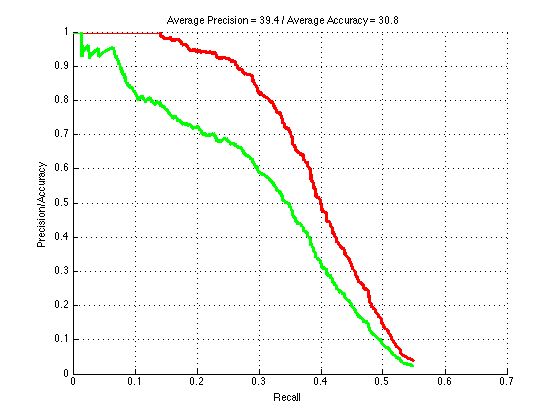
\includegraphics[width=\textwidth]{voc20128comp}
%                \caption{VOC2012 8 views}
%        \end{subfigure}
%        \begin{subfigure}[b]{0.49\textwidth}
%                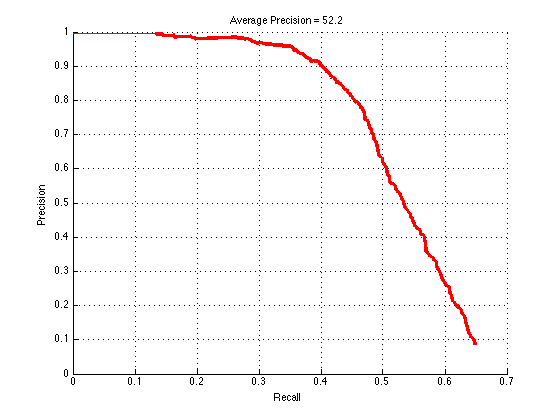
\includegraphics[width=\textwidth]{voc200716comp}
%               	\caption{VOC 2007 16 views}
%        \end{subfigure}
%        \begin{subfigure}[b]{0.49\textwidth}
%                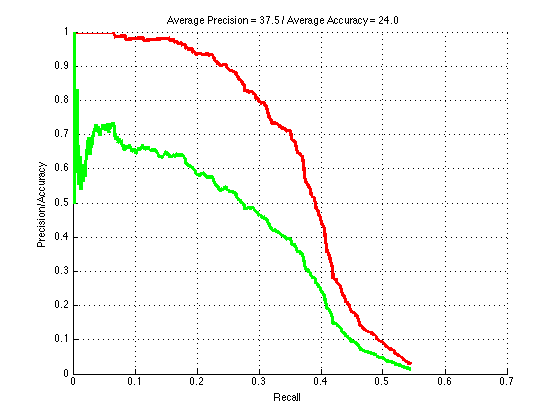
\includegraphics[width=\textwidth]{voc201216comp}
%                \caption{VOC2012 16 views}
%        \end{subfigure}        
%\caption{Precision-Recall curves of 3D-DPM on VOC 2007 'test' (left) and Precision/Accuracy-Recall curve on VOC 2012 'val' (right). }
%\label{fig:3ddpm}
%\end{center}
%\end{figure}
%
%\begin{figure}
%\begin{center}
%        \begin{subfigure}[b]{0.49\textwidth}
%                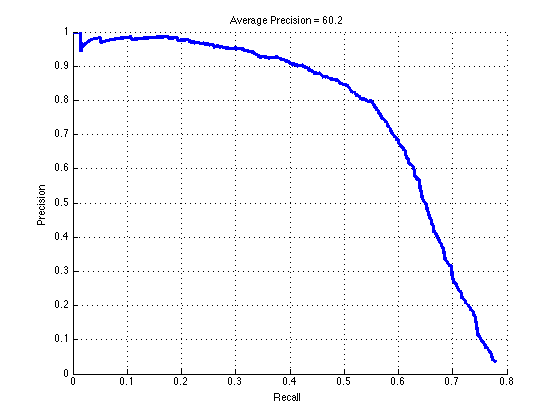
\includegraphics[width=\textwidth]{voc2007best4}
%               	\caption{VOC 2007 4 views}
%        \end{subfigure}
%        \begin{subfigure}[b]{0.49\textwidth}
%                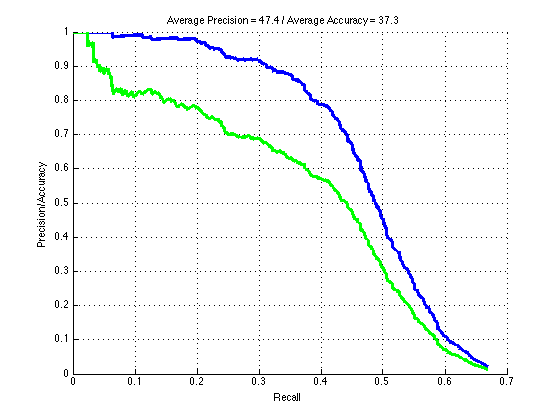
\includegraphics[width=\textwidth]{voc2012best4}
%                \caption{VOC2012 4 views}
%        \end{subfigure}
%        \begin{subfigure}[b]{0.49\textwidth}
%                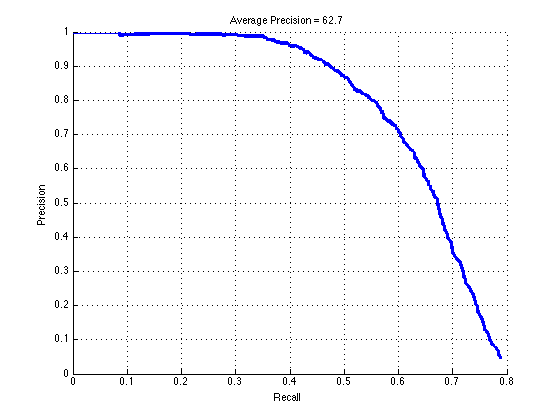
\includegraphics[width=\textwidth]{voc2007best8}
%               	\caption{VOC 2007 8 views}
%        \end{subfigure}
%        \begin{subfigure}[b]{0.49\textwidth}
%                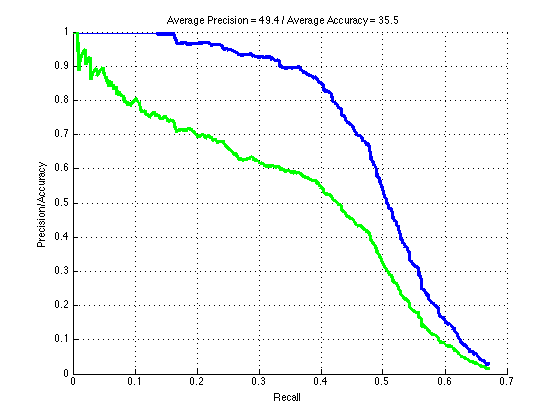
\includegraphics[width=\textwidth]{voc2012best8}
%                \caption{VOC2012 8 views}
%        \end{subfigure}
%        \begin{subfigure}[b]{0.49\textwidth}
%                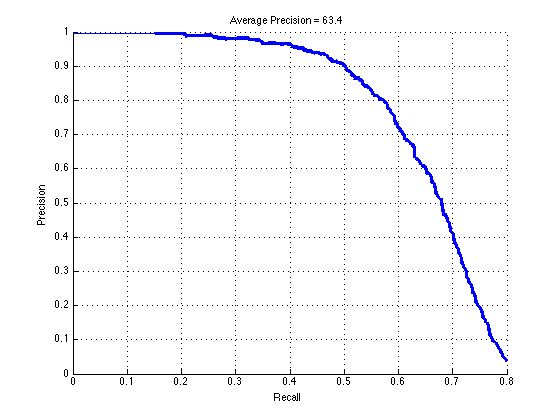
\includegraphics[width=\textwidth]{voc2007best16}
%               	\caption{VOC 2007 16 views}
%        \end{subfigure}
%        \begin{subfigure}[b]{0.49\textwidth}
%                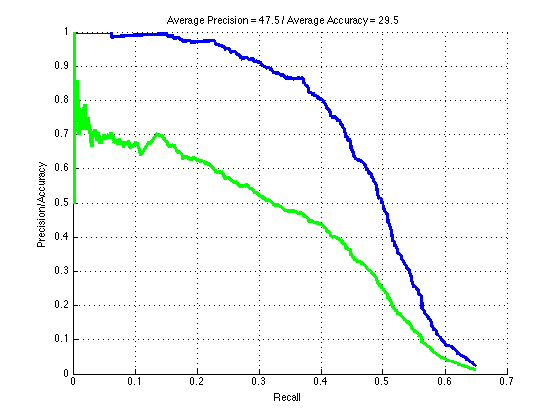
\includegraphics[width=\textwidth]{voc2012best16}
%                \caption{VOC2012 16 views}
%        \end{subfigure}        
%\caption{Precision-Recall curves of  3D-DPM+ on VOC 2007 'test' (left) and Precision/Accuracy-Recall curves on VOC 2012 'val' (right). }
%\label{fig:3ddpm+}
%\end{center}
%\end{figure}

% new PR figures

\begin{figure}
\begin{center}
	\begin{subfigure}[b]{0.49\textwidth}
       		\includegraphics[width=\textwidth]{3DdatasetPR}       
                \caption{3D-DPM}
        \end{subfigure}
        \begin{subfigure}[b]{0.49\textwidth}
       		\includegraphics[width=\textwidth]{3DdatasetVA}       
       		\caption{3D-DPM+}
        \end{subfigure}
%        \begin{subfigure}[b]{0.49\textwidth}
%       		\includegraphics[width=\textwidth]{3DdatasetPRbest}       
%                \caption{3D-DPM+}
%        \end{subfigure}
\caption{Precision/Recall (left) and Viewpoint-Accuracy/Recall (right) curves on cars of the 3D object dataset \cite{4408987} of models described in this project. All the models were trained using all the training data (CAD, VOC2007, VOC2012, 3D Dataset). 3D-DPM+ uses an extra octave pyramid and 3D-DPM PN uses positive training data with wrong viewpoint labels as negative training examples.}
\label{fig:PR3DDataset}
\end{center}
\end{figure}

\begin{figure}
\begin{center}
        \begin{subfigure}[b]{0.49\textwidth}
                \includegraphics[width=\textwidth]{voc2007PR4}
               	\caption{VOC 2007 4 views}
        \end{subfigure}
        \begin{subfigure}[b]{0.49\textwidth}
                \includegraphics[width=\textwidth]{voc2012PR4}
                \caption{VOC2012 4 views}
        \end{subfigure}
        \begin{subfigure}[b]{0.49\textwidth}
                \includegraphics[width=\textwidth]{voc2007PR8}
               	\caption{VOC 2007 8 views}
        \end{subfigure}
        \begin{subfigure}[b]{0.49\textwidth}
                \includegraphics[width=\textwidth]{voc2012PR8}
                \caption{VOC2012 8 views}
        \end{subfigure}
        \begin{subfigure}[b]{0.49\textwidth}
                \includegraphics[width=\textwidth]{voc2007PR16}
               	\caption{VOC 2007 16 views}
        \end{subfigure}
        \begin{subfigure}[b]{0.49\textwidth}
                \includegraphics[width=\textwidth]{voc2012PR16}
                \caption{VOC2012 16 views}
        \end{subfigure}        
\caption{Precision-Recall curves on VOC 2007 'test' (left) and on VOC 2012 'val' (right).  All the models were trained using all the training data.  }
\label{fig:PRVOC}
\end{center}
\end{figure}

\begin{figure}
\begin{center}
        \begin{subfigure}[b]{0.49\textwidth}
                \includegraphics[width=\textwidth]{voc2012VA4}
               	\caption{3D-DPM CNN 4 views}
        \end{subfigure}
        \begin{subfigure}[b]{0.49\textwidth}
                \includegraphics[width=\textwidth]{voc2012VA8}
               	\caption{3D-DPM CNN 8 views}
        \end{subfigure}
        \begin{subfigure}[b]{0.49\textwidth}
                \includegraphics[width=\textwidth]{voc2012VA16}
               	\caption{3D-DPM CNN 16 views}
        \end{subfigure}        
    \caption{Viewpoint-Accuracy-Recall curves on VOC 2012 'val' of models described in this project. Only examples with bounding-box overlap of at least 0.5 and correct viewpoint label are considered correctly classified. All the models were trained using all the training data (CAD, VOC2007, VOC2012, 3D Dataset). 3D-DPM+ uses an extra octave pyramid and 3D-DPM PN uses positive training data with wrong viewpoint labels as negative training examples.}
\label{fig:AVVOC2012}
\end{center}
\end{figure}

\section{Viewpoint Estimation}

To test the model's performance on pose-estimation, experiments on the 3D object dataset as well as the VOC 2012 'val' set with the viewpoint annotations from \cite{xiang_wacv14} were conducted. The performance measures used were viewpoint accuracy (VA) and mean precision in pose-estimation (MPPE). Viewpoint accuracy only counts detections with a minimum bounding box overlap of 50\% and a correct viewpoint assignment as valid detections, therefore measuring the combination of both, object localisation and viewpoint estimation. MPPE is defined as the average along the diagonal of the viewpoint confusion matrix, therefore ignoring correct bounding box localisation altogether. 

Table \ref{tab:voc2012} lists results on the 3D object category dataset in MPPE. 3D-DPM was trained using CAD renderings, examples from VOC 2012 and the first five cars of the 3D object category dataset. 3D-DPM+ again used all the training examples and makes use of an extra octave pyramid. Results for other 3D Deformable Parts Models  \cite{6248075} \cite{Pepik:2012aa} and DPM-VOC+VP \cite{6248075} are listed for comparison. Note however that the test sets might differ (see section  \ref{sec:boxloc}). The MPPE achieved by 3D-DPM is slightly higher than the results reported by the other 3D models and not quite as good as the results obtained by DPM-VOC+VP. Interestingly however, 3D-DPM+ performs worse than the other models on this dataset. 


The viewpoint accuracy results on VOC 2012 are listed in table \ref{tab:voc2012}. For comparison the results reported for DPM-VOC+VP and VDPM (DPMver4 initialised on correct viewpoints) are shown as well. By comparing the results of 3D-DPM to VDPM (which both use the same pyramid), we can observe the drastic improvement in viewpoint accuracy obtained by the continuous enforcement of correct viewpoints during training through component-fixation and the penalty term. The results for 3D-DPM+ show a significant improvement in viewpoint accuracy compared to 3D-DPM. This improvement is mainly due to the better detection performance and does not imply that 3D-DPM+ obtains better viewpoint estimation given a correct detection. The results achieved by  3D-DPM+ are nearly identical to the results obtained by DPM-VOC+VP \cite{6248075}.

\section{CNN vs. HOG Features}\label{sec:cnnexp}	

This section will present the influence of several design choices on the performance of a CNN based model, report results obtained with such models and compare the performance of a CNN based model to HOG based models. 

\begin{table}[]
	\begin{center}
		\begin{tabular}{|c|c|c|}
		\hline
		Feature standardisation & AP & VA\\
		\hline\hline
		 without & 0 & 0\\
		\hline 
		 with & +22 & +21.5 \\
		 \hline 
		\end{tabular}
	\end{center}
	\caption{Relative AP and VA with or without feature standardisation}
	\label{tab:featStand}
\end{table}

\begin{table}[]
	\begin{center}
		\begin{tabular}{|c|c|c|}
		\hline
		Lower bounds on deformations & AP & VA\\
		\hline\hline
		 $(0.01, 0, 0.01, 0)$ & 0 & 0\\
		\hline 
		 $(0.2, 0, 0.2, 0)$ & +7.6 & +8.4 \\
		 \hline 
		\end{tabular}
	\end{center}
	\caption{Relative AP and VA for different lower-bounds}
	\label{tab:lowerbound}
\end{table}

Table \ref{tab:featStand} lists the relative performance gain on the VOC2012 'val' set achieved through feature standardisation and table \ref{tab:lowerbound} shows the influence of the increased deformation lower-bounds. The importance of these modifications is obvious from the experiments. As mentioned in section \ref{sec:cnnFeat}, feature standardisation mainly improves the SVM training while the increased lower-bounds are important to prevent parts from moving too far away from their anchor positions. 

\begin{table}[]
	\begin{center}
		\begin{tabular}{|c|c|c|}
		\hline
		\#views & 3D-DPM CNN & 3D-DPM HOG\\
		\hline\hline
		4 &  55.3  & 54.3\\
		\hline
		8 & 53.1 &  54.7\\
		\hline
		16 & 51.8 &  57.1 \\
		\hline
		\end{tabular}
	\end{center}
\caption{Comparing the detection performance of a CNN based model to a HOG based model using average precision on cars of the VOC 2007 'test' set.}\label{tab:cnn2007}
\end{table}

%\begin{figure}
%\begin{center}
%        \begin{subfigure}[b]{0.49\textwidth}
%                \includegraphics[width=\textwidth]{voc2007PRcnn4}
%               	\caption{3D-DPM CNN 4 views}
%        \end{subfigure}
%        \begin{subfigure}[b]{0.49\textwidth}
%                \includegraphics[width=\textwidth]{voc2007PRcnn8}
%               	\caption{3D-DPM CNN 8 views}
%        \end{subfigure}
%        \begin{subfigure}[b]{0.49\textwidth}
%                \includegraphics[width=\textwidth]{voc2007PRcnn16}
%               	\caption{3D-DPM CNN 16 views}
%        \end{subfigure}        
%    \caption{Precision/Accuracy-Recall curves on VOC 2007 'test' of 3D-DPM CNN (left) and 3D-DPM CNN-PN (right). }
%\label{fig:voc2007cnn}
%\end{center}
%\end{figure}

Results for a CNN-based model on VOC 2007 'test' are listed in table \ref{tab:cnn2007}. For comparison, the results of a HOG-based 3D-DPM are also shown. Both these models were trained using all the training data. 3D-DPM CNN is trained using badly localised positives as negatives in addition to the normal negative training examples. Only positive examples with annotated bounding box overlap of less than 30\% count as badly localised and care is taken to only consider images where not more than one car is present to extract negative examples from. We can observe that the CNN model only performs better with a four-viewpoints-model. Note how the performance of 3D-DPM CNN decreases with an increased number of model viewpoints, while the performance of the HOG model improves. This observation was also made on other datasets and probably has to do with the reduction of training data for each individual model viewpoint. 


\begin{table}[]
	\begin{center}
		\begin{tabular}{|c|c|c|c|}
		\hline
		\#views & 3D-DPM CNN & 3D-DPM CNN-PN & 3D-DPM HOG\\
		\hline\hline
		4 &  38.0/24.4 & 34.1/28.0 & 38.2/30.2\\
		\hline
		8 & 38.0/23.8  & 35.1/26.8 &  39.4/30.8\\
		\hline
		16 & 35.2/14.6 & 30.9/17.8 & 37.5/24.0\\
		\hline
		\end{tabular}
	\end{center}
\caption{Comparing the performance of CNN based models to a HOG based model using average precision and average viewpoint accuracy (AP/VA) on cars of the VOC 2012 'val' set with annotations by \cite{xiang_wacv14}.}\label{tab:cnn2012}
\end{table}

%\begin{figure}
%\begin{center}
%        \begin{subfigure}[b]{0.49\textwidth}
%                \includegraphics[width=\textwidth]{voc2012PRcnn4}
%               	\caption{3D-DPM CNN 4 views}
%        \end{subfigure}
%        \begin{subfigure}[b]{0.49\textwidth}
%                \includegraphics[width=\textwidth]{voc2012PRcnnPN4}
%                \caption{3D-DPM CNN-PN 4 views}
%        \end{subfigure}
%        \begin{subfigure}[b]{0.49\textwidth}
%                \includegraphics[width=\textwidth]{voc2012PRcnn8}
%               	\caption{3D-DPM CNN 8 views}
%        \end{subfigure}
%        \begin{subfigure}[b]{0.49\textwidth}
%                \includegraphics[width=\textwidth]{voc2012PRcnnPN8}
%                \caption{3D-DPM CNN-PN 8 views}
%        \end{subfigure}
%        \begin{subfigure}[b]{0.49\textwidth}
%                \includegraphics[width=\textwidth]{voc2012PRcnn16}
%               	\caption{3D-DPM CNN 16 views}
%        \end{subfigure}
%        \begin{subfigure}[b]{0.49\textwidth}
%                \includegraphics[width=\textwidth]{voc2012PRcnnPN16}
%                \caption{3D-DPM CNN-PN 16 views}
%        \end{subfigure}        
%\caption{Precision/Accuracy-Recall curves on VOC 2012 'val' of 3D-DPM CNN (left) and 3D-DPM CNN-PN (right). }
%\label{fig:voc2012cnn}
%\end{center}
%\end{figure}

In table \ref{tab:cnn2012} the performance of two CNN based models on VOC2012 'val' are shown in comparison to the HOG based 3D-DPM. The HOG based model doesn't make use of an extra octave, therefore making the feature pyramids of all the models comparable relative to their root size.  We can observe that the detection performance of 3D-DPM CNN is only slightly below the performance achieved  by 3D-DPM HOG. This is in accordance with recent work combining CNN features with DPMs \cite{girshick2014deformable} where the car category has shown to be one of only two categories where AP did not increase with CNN features while significantly improving the mean average precision (mAP) over all object categories (from 33.7 for HOG to 44.4 for CNN on VOC2007). While average precision is about on par with HOG based models, we can see that the viewpoint accuracy (VA) of 3D-DPM CNN is several points below the VA achieved by 3D-DPM HOG. This is due to a tendency observed in CNN based models to assign examples that are not viewpoint annotated to only a few model components. This results in detections that are concentrated on only those few components. As VA is arguably a better measure for the performance of a 3D-DPM as it directly measures the two main objectives of a 3D-DPM (object localisation and pose-estimation) we would like to increase the models VA performance. 3D-DPM CNN-PN uses positive examples with wrong viewpoint assignments as additional negative training examples. The intuition is that the model in this case learns to better distinguish between the different viewpoints of the object. As can be seen in table \ref{tab:cnn2012} the VA clearly improves with this training procedure while AP significantly decreases, and VA still not matching the performance of 3D-DPM HOG. %Figure \ref{fig:voc2012cnn} presents PR curves for the two CNN-based models on VOC 2012 'val'.


\begin{table}[]
	\begin{center}
		\begin{tabular}{|c|c|c|}
		\hline
		3D-DPM CNN & 3D-DPM CNN-PN & 3D-DPM HOG\\
		\hline\hline
		97.9/82.8 & 97.6/97.5 & 99.14/93.0\\
		\hline
		\end{tabular}
	\end{center}
\caption{Comparing the performance of CNN based models to a HOG based model using average precision and average viewpoint accuracy (AP/VA) on cars of the 3D object dataset \cite{4408987}.}\label{tab:cnn3ddataset}
\end{table}

%\begin{figure}
%\begin{center}
%	\begin{subfigure}[b]{0.49\textwidth}
%       		\includegraphics[width=\textwidth]{3ddataPRcnn}       
%                \caption{3D-DPM CNN}
%        \end{subfigure}
%        \begin{subfigure}[b]{0.49\textwidth}
%       		\includegraphics[width=\textwidth]{3ddataPRcnnPN}       
%                \caption{3D-DPM CNN-PN}
%        \end{subfigure}
%\caption{Precision/Recall and Viewpoint-Accuracy/Recall curves on cars of the 3D object dataset \cite{4408987}.}
%\label{fig:3ddataPRcnn}
%\end{center}
%\end{figure}

It is interesting to note however the results achieved on the 3D object dataset \cite{4408987} (listed in table \ref{tab:cnn3ddataset}). This dataset contains only cars in full sight, i.e. no truncated or occluded cars. Here 3D-DPM CNN-PN achieves the highest VA of all the models, also clearly outperforming the HOG based model. It is also noteworthy that AP and VA are nearly identical for 3D-DPM CNN-PN, therefore achieving the highest VA/AP ratio of all the models (see figure \ref{fig:PR3DDataset}).

Overall, the observation is that off-the-shelf CNN features do not lead to better results for 3D Deformable Parts Models on cars. It should be noted that the features used here were trained for image classification and that fine-tuning the parameters for object detection usually results in rather drastic performance improvements. 




\chapter{Conclusion}\label{chap:conclusion} 
During this project a 3D Deformable Parts Model was implemented and carefully evaluated with respect to different design choices and model parameters. The result of this work is a 3D model whose performance on object detection and pose-estimation is on par and in many cases even better than results reported for other 3D-DPMs \cite{Pepik:2012aa} \cite{6248075}. Through the evaluation of several design choices and model parameters, deeper insights into the training of 3D-DPMs and DPMs in general have  been gained. Among the factors that turned out to be important, were the construction of the feature pyramid where an extra octave (to detect small objects) showed significant performance improvements. The way how truncated and occluded objects are handled turned out to be crucial as well, and it was found that performance improves significantly by the use of a truncation feature and effective handling of bounding-box overlap requirements during training. It has also been shown how different types of CAD examples affect the performance of the model. Here, perspective renderings on uniform backgrounds have proofed to work best. The introduction of a penalty term during latent positive search has turned out to be an effective way to increase the viewpoint accuracy of the 3D-DPM.

While the model has shown to perform well on viewpoint estimation, the estimations at the moment are still limited to a set of discrete viewpoints the model was trained on. While it is in theory possible to train the model on arbitrarily many discrete viewpoints (provided that sufficient CAD renderings are generated), this is clearly not an efficient solution. An idea for a new and alternative approach is outlined in section \ref{sec:future}.

The incorporation of features obtained by Convolutional Neural Networks has been found to be more difficult than expected. Feature standardisation, an adjustment of the deformation lower-bounds and a modification of the training procedure have proofed to be essential to get a comparable detection performance to HOG features. Also some compromise between performance and training time had to be made in order to make experiments feasible (reducing the number of pyramid levels mainly). While the detection performance of HOG features can nearly be matched by CNN based models using these modifications, the viewpoint estimation capabilities of CNN based models showed to be significantly worse. By using wrong viewpoint assignments as negative examples during training, I managed to increase the pose-estimation performance with CNN features such that they even exceed the performance of HOG based models on datasets where objects are not occluded or truncated. 

%There were several challenges to be mastered during the work on this project. The first (and probably the most overwhelming) being getting to know and understand the rather complex implementation of the DPM. This was crucial though as making modifications to the code very often affected several other portions of it, which had to be adjusted or modified.  I tried to refactor the code in several ways to make it more modular and flexible. The lesson learned here is, that code, which is well designed with respect to clearly stated and distributed responsibilities, greatly simplifies modifications. 
%
%Looking back, another lesson learned during the work on the project is that of verifying modifications after they have been applied. Too long I was working on the code, making several often massive changes, without controlling their effect on the model's performance. Of course I made sure that it still runs error free, but this does  This of course made finding and solving "bugs" unnecessarily more difficult than it would have been if rigorous tests would have been performed after each major modification. The time needed for training and evaluating a model on a PC however often discouraged such tests and I only really started with such rigorous testing when working on the cluster.  

\section{Future work}\label{sec:future}
One idea of future research work on the model  aims to increase the model's viewpoint accuracy, and to also allow for finer viewpoint estimation. Rather than using interpolation between filters at test-time to allow finer viewpoint estimation  as in \cite{Pepik:2012aa} (which increases detection time), the idea is to use a voting scheme to determine the viewpoint. Given an image of a car, there are typically going to be several overlapping object hypotheses with different viewpoint assignments and scores around the correct object localisation. Rather than just applying non-maximal suppression on all these hypotheses, the non-maximal suppression could only be applied to groups of possible detections with the same viewpoint-assignment only and the resulting set of hypotheses used to arrive at a better, more complete object hypothesis. The most confident (highest scoring) hypothesis  could  be used as an initial guess for the viewpoint and location of the object and hypotheses with neighbouring viewpoints as well as a certain overlap with the initial guess could then be used to refine the initial guess by voting for other viewpoints (with voting-weights  being proportional to the hypothesis score). This approach would also not lead to a significant increase in detection time as there are not more convolutions of the filters with the feature maps needed. 

Another path for future work could be the improvement of the CNN based models by fine-tuning the network weights to the given task of object detection with Deformable Parts Models. As such fine-tuning has shown to be very effective by \cite{girshick2013rich}, this could result in much better performance. To adapt the fine-tuning procedure to the intended use with DPMs, region proposals with a bounding box overlap of more than 0.5 as well as smaller regions totally inside the bounding box (related to possible parts) could be used as positive examples. 

It would also be interesting to test the models performance on other object classes, especially with CNN features as they have shown to improve over HOG features for other object classes than cars. This of course means that training data in the form of CAD examples would first have to be created. 

\bibliographystyle{plain} %apalike
\bibliography{refs}

\appendix
\chapter{Image and Feature Pyramid}\label{chap:pyra} 
Sliding window approaches make use of feature pyramids to detect objects at different scales and locations in an image. To compute a  feature pyramid, first an image pyramid is constructed. Image pyramids are constructed via repeated subsampling of the original image. The subsampling factor between any two consecutive pyramid levels is constant and determined via a parameter $\lambda$. This parameter $\lambda$ defines the number of levels in an octave. An octave in turn is defined as the number of levels that have to be stepped down in a pyramid until an image of twice the resolution is reached. Figure \ref{fig:impyra} visualises an image pyramid with two octaves and $\lambda=1$. The bottom level of an image pyramid is usually at twice the resolution of the original image. In case an extra-octave pyramid or CNN features are used, the original image is resized to twice the resolution before the construction of the image pyramid, which results in a bottom level that has four times the resolution of the original image. Note that only the parts will be placed in the higher resolution bottom octave of the pyramid. After the image pyramid is constructed, feature maps are computed for every pyramid level which results in the desired feature pyramid (see figure \ref{fig:featpyra}).

\end{document}